\documentclass{article}

% packages
  % basic stuff for rendering math
  \usepackage[letterpaper, top=1in, bottom=1in, left=1in, right=1in]{geometry}
  \usepackage[utf8]{inputenc}
  \usepackage[english]{babel}
  \usepackage{amsmath} 
  \usepackage{amssymb}

  % extra math symbols and utilities
  \usepackage{mathtools}        % for extra stuff like \coloneqq
  \usepackage{mathrsfs}         % for extra stuff like \mathsrc{}
  \usepackage{centernot}        % for the centernot arrow 
  \usepackage{bm}               % for better boldsymbol/mathbf 
  \usepackage{enumitem}         % better control over enumerate, itemize
  \usepackage{hyperref}         % for hypertext linking
  \usepackage{fancyvrb}          % for better verbatim environments
  \usepackage{newverbs}         % for texttt{}
  \usepackage{xcolor}           % for colored text 
  \usepackage{listings}         % to include code
  \usepackage{lstautogobble}    % helper package for code
  \usepackage{parcolumns}       % for side by side columns for two column code
  

  % page layout
  \usepackage{fancyhdr}         % for headers and footers 
  \usepackage{lastpage}         % to include last page number in footer 
  \usepackage{parskip}          % for no indentation and space between paragraphs    
  \usepackage[T1]{fontenc}      % to include \textbackslash
  \usepackage{footnote}
  \usepackage{etoolbox}

  % for custom environments
  \usepackage{tcolorbox}        % for better colored boxes in custom environments
  \tcbuselibrary{breakable}     % to allow tcolorboxes to break across pages

  % figures
  \usepackage{pgfplots}
  \pgfplotsset{compat=1.18}
  \usepackage{float}            % for [H] figure placement
  \usepackage{tikz}
  \usepackage{tikz-cd}
  \usepackage{circuitikz}
  \usetikzlibrary{arrows}
  \usetikzlibrary{positioning}
  \usetikzlibrary{calc}
  \usepackage{graphicx}
  \usepackage{algorithmic}
  \usepackage{caption} 
  \usepackage{subcaption}
  \captionsetup{font=small}

  % for tabular stuff 
  \usepackage{dcolumn}

  \usepackage[nottoc]{tocbibind}
  \pdfsuppresswarningpagegroup=1
  \hfuzz=5.002pt                % ignore overfull hbox badness warnings below this limit

% New and replaced operators
  \DeclareMathOperator{\Tr}{Tr}
  \DeclareMathOperator{\Sym}{Sym}
  \DeclareMathOperator{\Span}{span}
  \DeclareMathOperator{\std}{std}
  \DeclareMathOperator{\Cov}{Cov}
  \DeclareMathOperator{\Var}{Var}
  \DeclareMathOperator{\Corr}{Corr}
  \DeclareMathOperator{\pos}{pos}
  \DeclareMathOperator*{\argmin}{\arg\!\min}
  \DeclareMathOperator*{\argmax}{\arg\!\max}
  \newcommand{\ket}[1]{\ensuremath{\left|#1\right\rangle}}
  \newcommand{\bra}[1]{\ensuremath{\left\langle#1\right|}}
  \newcommand{\braket}[2]{\langle #1 | #2 \rangle}
  \newcommand{\qed}{\hfill$\blacksquare$}     % I like QED squares to be black

% Custom Environments
  \newtcolorbox[auto counter, number within=section]{question}[1][]
  {
    colframe = orange!25,
    colback  = orange!10,
    coltitle = orange!20!black,  
    breakable, 
    title = \textbf{Question \thetcbcounter ~(#1)}
  }

  \newtcolorbox[auto counter, number within=section]{exercise}[1][]
  {
    colframe = teal!25,
    colback  = teal!10,
    coltitle = teal!20!black,  
    breakable, 
    title = \textbf{Exercise \thetcbcounter ~(#1)}
  }
  \newtcolorbox[auto counter, number within=section]{solution}[1][]
  {
    colframe = violet!25,
    colback  = violet!10,
    coltitle = violet!20!black,  
    breakable, 
    title = \textbf{Solution \thetcbcounter}
  }
  \newtcolorbox[auto counter, number within=section]{lemma}[1][]
  {
    colframe = red!25,
    colback  = red!10,
    coltitle = red!20!black,  
    breakable, 
    title = \textbf{Lemma \thetcbcounter ~(#1)}
  }
  \newtcolorbox[auto counter, number within=section]{theorem}[1][]
  {
    colframe = red!25,
    colback  = red!10,
    coltitle = red!20!black,  
    breakable, 
    title = \textbf{Theorem \thetcbcounter ~(#1)}
  } 
  \newtcolorbox[auto counter, number within=section]{proposition}[1][]
  {
    colframe = red!25,
    colback  = red!10,
    coltitle = red!20!black,  
    breakable, 
    title = \textbf{Proposition \thetcbcounter ~(#1)}
  } 
  \newtcolorbox[auto counter, number within=section]{corollary}[1][]
  {
    colframe = red!25,
    colback  = red!10,
    coltitle = red!20!black,  
    breakable, 
    title = \textbf{Corollary \thetcbcounter ~(#1)}
  } 
  \newtcolorbox[auto counter, number within=section]{proof}[1][]
  {
    colframe = orange!25,
    colback  = orange!10,
    coltitle = orange!20!black,  
    breakable, 
    title = \textbf{Proof. }
  } 
  \newtcolorbox[auto counter, number within=section]{definition}[1][]
  {
    colframe = yellow!25,
    colback  = yellow!10,
    coltitle = yellow!20!black,  
    breakable, 
    title = \textbf{Definition \thetcbcounter ~(#1)}
  } 
  \newtcolorbox[auto counter, number within=section]{example}[1][]
  {
    colframe = blue!25,
    colback  = blue!10,
    coltitle = blue!20!black,  
    breakable, 
    title = \textbf{Example \thetcbcounter ~(#1)}
  } 
  \newtcolorbox[auto counter, number within=section]{code}[1][]
  {
    colframe = green!25,
    colback  = green!10,
    coltitle = green!20!black,  
    breakable, 
    title = \textbf{Code \thetcbcounter ~(#1)}
  } 
  \newtcolorbox[auto counter, number within=section]{algo}[1][]
  {
    colframe = green!25,
    colback  = green!10,
    coltitle = green!20!black,  
    breakable, 
    title = \textbf{Algorithm \thetcbcounter ~(#1)}
  } 

  \BeforeBeginEnvironment{example}{\savenotes}
  \AfterEndEnvironment{example}{\spewnotes}
  \BeforeBeginEnvironment{lemma}{\savenotes}
  \AfterEndEnvironment{lemma}{\spewnotes}
  \BeforeBeginEnvironment{theorem}{\savenotes}
  \AfterEndEnvironment{theorem}{\spewnotes}
  \BeforeBeginEnvironment{corollary}{\savenotes}
  \AfterEndEnvironment{corollary}{\spewnotes}
  \BeforeBeginEnvironment{proposition}{\savenotes}
  \AfterEndEnvironment{proposition}{\spewnotes}
  \BeforeBeginEnvironment{definition}{\savenotes}
  \AfterEndEnvironment{definition}{\spewnotes}
  \BeforeBeginEnvironment{exercise}{\savenotes}
  \AfterEndEnvironment{exercise}{\spewnotes}
  \BeforeBeginEnvironment{proof}{\savenotes}
  \AfterEndEnvironment{proof}{\spewnotes}
  \BeforeBeginEnvironment{solution}{\savenotes}
  \AfterEndEnvironment{solution}{\spewnotes}
  \BeforeBeginEnvironment{question}{\savenotes}
  \AfterEndEnvironment{question}{\spewnotes}
  \BeforeBeginEnvironment{code}{\savenotes}
  \AfterEndEnvironment{code}{\spewnotes}
  \BeforeBeginEnvironment{algo}{\savenotes}
  \AfterEndEnvironment{algo}{\spewnotes}

  \definecolor{dkgreen}{rgb}{0,0.6,0}
  \definecolor{gray}{rgb}{0.5,0.5,0.5}
  \definecolor{mauve}{rgb}{0.58,0,0.82}
  \definecolor{darkblue}{rgb}{0,0,139}
  \definecolor{lightgray}{gray}{0.93}
  \renewcommand{\algorithmiccomment}[1]{\hfill$\triangleright$\textcolor{blue}{#1}}

  % default options for listings (for code)
  \lstset{
    autogobble,
    frame=ltbr,
    language=Python,
    aboveskip=3mm,
    belowskip=3mm,
    showstringspaces=false,
    columns=fullflexible,
    keepspaces=true,
    basicstyle={\small\ttfamily},
    numbers=left,
    firstnumber=1,                        % start line number at 1
    numberstyle=\tiny\color{gray},
    keywordstyle=\color{blue},
    commentstyle=\color{dkgreen},
    stringstyle=\color{mauve},
    backgroundcolor=\color{lightgray}, 
    breaklines=true,                      % break lines
    breakatwhitespace=true,
    tabsize=3, 
    xleftmargin=2em, 
    framexleftmargin=1.5em, 
    stepnumber=1
  }

% Page style
  \pagestyle{fancy}
  \fancyhead[L]{Image and Video Processing}
  \fancyhead[C]{Muchang Bahng}
  \fancyhead[R]{Fall 2023} 
  \fancyfoot[C]{\thepage / \pageref{LastPage}}
  \renewcommand{\footrulewidth}{0.4pt}          % the footer line should be 0.4pt wide
  \renewcommand{\thispagestyle}[1]{}  % needed to include headers in title page

\begin{document}

\title{Image and Video Processing}
\author{Muchang Bahng}
\date{Fall 2023}

\maketitle
\tableofcontents
\pagebreak

\section{Introduction to Image and Video Processing}

    Image and video processing has applications in outer space, medical procedures, and consumer brands. The spectrum of light for which we can see with our naked eye is a very small portion of the entire spectrum. Therefore, image processing goes much beyond what we can see with our eyes, and in some cases, we would take multiple images from multiple wavelengths of the same scene to discern different types of information from them. 

    \begin{center}
        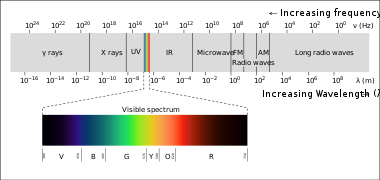
\includegraphics[scale=0.7]{img/em_spectrum.png}
    \end{center}

  \subsection{Human Visual System}

    The human eye has cones (used for eyeing details and good at seeing in high light) and rods (used for eyeing general scenes and good at seeing in low light). The light comes in through out cornea and lens, and projects it into our retina. There is a blind spot where there are no receptors. With the cones and rods, we can see in a very broad range of light intensities. 
    \begin{center}
        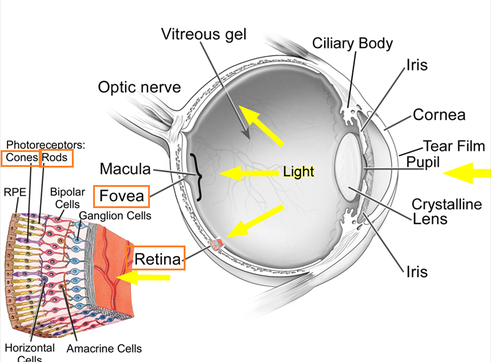
\includegraphics[scale=0.4]{img/eye_diagram.png}
    \end{center}
    There are certain laws of the human visual system: 
    \begin{enumerate}
        \item \textbf{Weber law} says that we have a harder time distinguishing objects that are very dark (slight changes in brightness in a dark environment will not be perceived) than objects in light conditions. Therefore, \textbf{brightness adaptation} is needed when adjusting to new environments. 
        
        \item \textbf{Mach bands} is an optical illusion that exaggerates the contrast between edges of slightly differing shades of gray, as soon as they contact on another, by triggering edge-detection in the human visual system. 
        \begin{center}
            
\includegraphics[scale=0.4]{img/mach_bands.png}
        \end{center}
    \end{enumerate}

  \subsection{Image Formation: Sampling and Quantization}

    Now when we have a scene, which is a continuous image, we need to make sure that the image fits the resolution. This is done in two ways: 
    \begin{enumerate}
      \item \textbf{Discretization}, or \textbf{sampling}, in the spatial domain, i.e. fitting everything into a $N \times M$ resolution. This tells you how fine the sampling is within the continuous image. 
      \item \textbf{Quantization} in the color, i.e. quantizing the values into $[255]$ for grayscale (by representing colors in 8 bits, so $2^8$ colors) and $[255]^3$ for RGB color. Another thing to note is that when you take an image which has 8 bits per pixel, so 256 values, you can use further quantization to compress it into say 7 bits by doing the operation 
      \[\lfloor x/2 \rfloor \times 2\]
      which maps $2x, 2x + 1 \mapsto 2x$. However, too much quantization may lead to too many pixel colors being pushed to 255 and leaving large chunks of white in the image, called \textbf{saturation}. 
    \end{enumerate}
    \begin{center}
        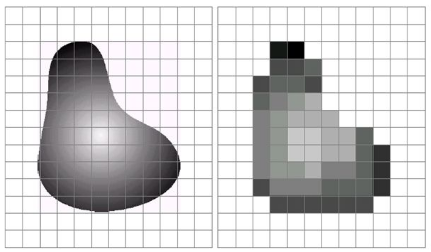
\includegraphics[scale=0.4]{img/discretization_quantization.png}
    \end{center}
    For high quality cameras, they store all 3 separate channels for RGB: 3 images. 
    \begin{center}
        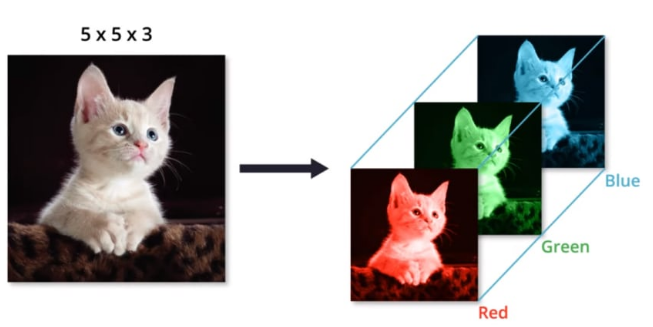
\includegraphics[scale=0.3]{img/RGB_channels.png}
    \end{center}
    However, mosaic cameras alternate between RGB in the images, storing 1/3 R 1/3 B 1/3 G in one image for better compression, called a \textbf{bayer filter}. 
    \begin{center}
        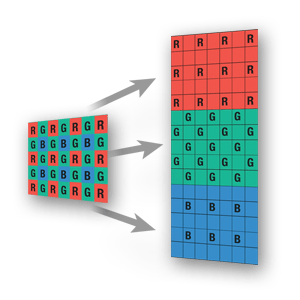
\includegraphics[scale=0.3]{img/bayer_filter.png}
    \end{center}

    Now at this point, we can interpret an image as a matrix or a 3-tensor Therefore, we can do simple operations like addition, subtraction, inverse, etc. We could rotate them too. 

\section{Image and Video Compression}

    Now let's talk about how these are stored. If we have a resolution of $N \times M$, along with a quantization of $B$ bits, then for each pixel in the image, we can take a total of $2^B$ different values. Therefore, 
    \begin{enumerate}
        \item For an grayscale image, the total number of bits that we would need to store it is $NMB$. 
        \item If we are working with color images, then there are three channels, so we need $3NMB$ bits. 
        \item When looking at a video that records at $F$ frames per second, that is $S$ seconds long, then have a total of $FS$ images, and so for a colored video we need $23NMB \times FS$ bits. 
    \end{enumerate}
    This is clearly a lot of bits and can easily exceed many gigabytes. Therefore, the vast majority of images are compressed using different standards (JPEG, JPEG-LS, JPEG-2000), along with videos (MPEG). It follows the structure: 
    \begin{center}
        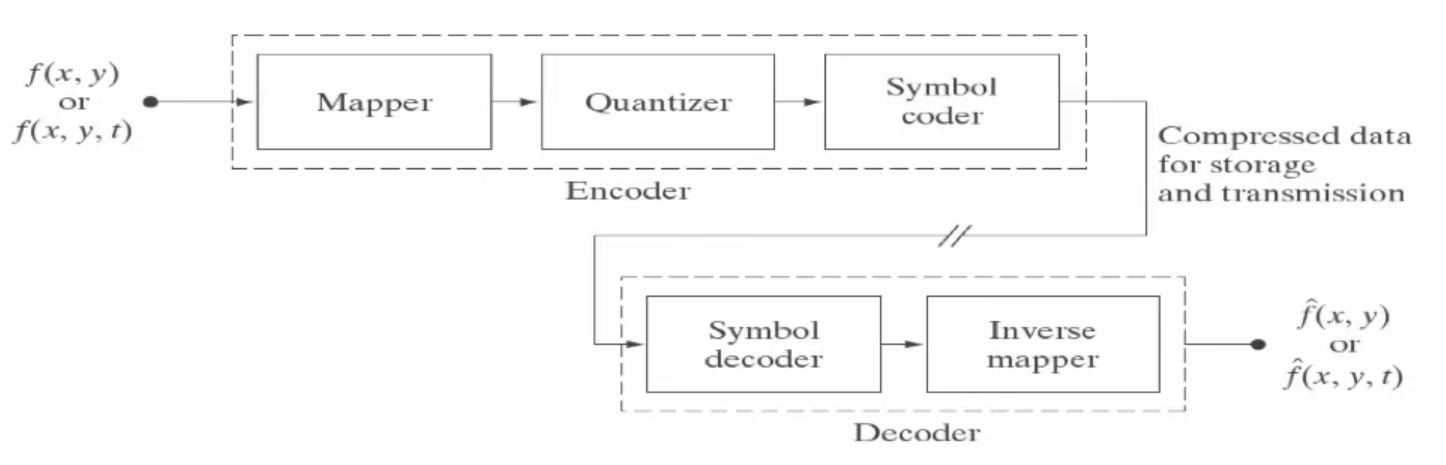
\includegraphics[scale=0.27]{img/JPEG.png}
    \end{center}
    We describe the steps below, but focus specifically on the JPEG standard. 
    \begin{enumerate}
        \item Before any of this happens, JPEG actually takes the image and constructs $n \times n$ subimages that are each put through the pipeline. It is usually $n = 8$. 
        \item The \textbf{mapper} takes in the array and transforms it in a way that is more friendly to compression. In JPEG, we use the discrete cosine transform (DCT). 
        \item After the mapping, we do quantization on the image. This is the main source of error, but it transforms the image into something that is more friendly for symbol decoding. More specifically, the quantization makes sure that the distribution of pixel values are very concentrated so that we can use Huffman coding to compress the image by a lot. 
        \item The symbol encoder then encodes each pixel into shorter lengths. Huffman encoding is used. 
    \end{enumerate}

  \subsection{Frontend: N x N Block Division of Image}

    For color images, JPEG transforms every RGB 3-pixels into $Y C_B C_R$ (where $Y$ represents the luminance), which is represented by a linear map: 
    \[\begin{pmatrix} Y  \\ C_B \\ C_R \end{pmatrix} = \begin{pmatrix} & & \\ & A & \\ & & \end{pmatrix} \begin{pmatrix} R \\ G \\ B \end{pmatrix} \]
    and then it divides into the $8 \times 8$ blcoks. So, we have a bunch of $8 \times 8$ blocks of pixels in $Y C_B C_R$ format. 

  \subsection{Forward Transform: DCT}

    Imagine you have an $N \times N$ image with pixels labeled $f(x, y)$. Then, we want to get a new image $T$ with the following transform. 
    \[T(u, v) = \sum_{x=0}^{n-1} \sum_{y=0}^{n-1} f(x, y) \, r(x, y, u, v)\]
    This can be inverted with the inverse transform 
    \[f(x, y) = \sum_{u=0}^{n-1} \sum_{v=0}^{n-1} T(u, v) \, s(x, y, u, v)\]
    To specify the transform, I just need to tell you $r$ and $s$ s.t. it minimizes some mean squared error. In DCT, we have 
    \[r(x, y, u, v) = s(x, y, u, v) = \alpha(u) \, \alpha(v) \cos \bigg[ \frac{(2x + 1) u \pi}{2 n} \bigg] \cos \bigg[ \frac{(2 y + 1) v \pi}{2 n} \bigg]\]
    where 
    \[\alpha (u) = \begin{cases} \sqrt{1/n} & \text{ if } u = 0 \\ \sqrt{2/n} & \text{ if } v = 0 \end{cases}\]
    is a normalization term. It is clear that $r$ and $s$ are some basis functions, and you are representing your image into a linear combination of simple ``cosine" images. For every fixed $(u, v)$, we have $(x, y) \in [u]^2$ which forms an image, and this basis is always fixed. 
    \begin{center}
        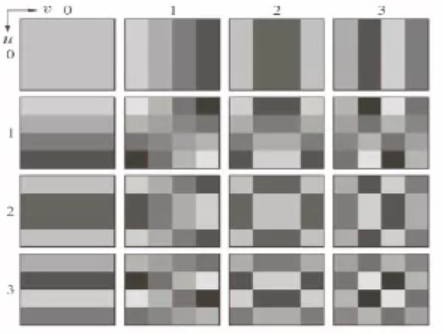
\includegraphics[scale=0.4]{img/cosine_transform.png}
    \end{center}

    There are two reasons we prefer DCT: 
    \begin{enumerate}
        \item It has a nice periodicity assumption that is more applicable. 
        \item Under Markovian assumptions, DCT coincides with the Kosambi–Karhunen–Loève transform. 
    \end{enumerate}

  \subsection{Quantization}

  \subsection{Huffman Coding}

    To do Huffman coding, imagine you have an image with just 4 different pixel colors. 
    \begin{center}
        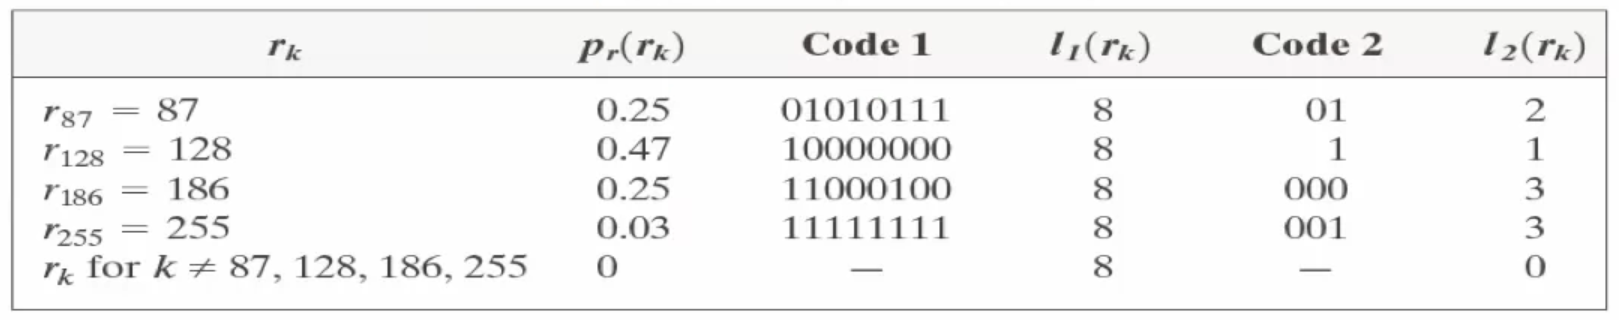
\includegraphics[scale=0.25]{img/pixels_huffman.png}
    \end{center}
    The length of every pixel is $8$ bits, so the expected length of each pixel is $8$. However, if we do Huffman encoding, we are basically creating a binary tree by taking the two pixels with the lowest proportion and summing them up to get a new proportion, and simply repeating these steps. This creates a prefix free code. 
    \begin{enumerate}
        \item We start with the 2 smallest probabilities 
        \item Add them to the root node and then look for the next 2 smallest. 
    \end{enumerate}
    \begin{center}
        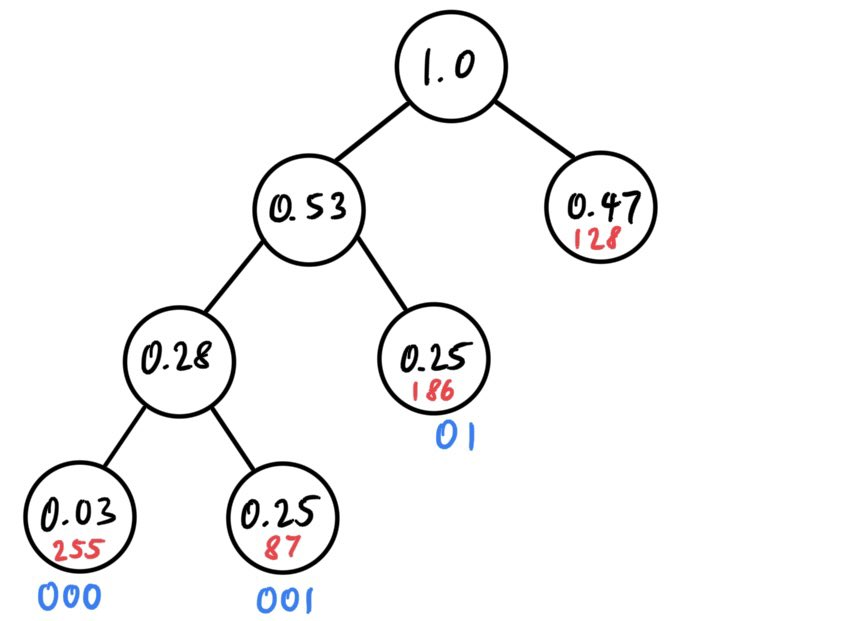
\includegraphics[scale=0.25]{img/huffman.png}
    \end{center}
    Therefore, the expected number of bits needed now is 
    \[0.25 \cdot 2 + 0.47 \cdot 1 + 0.25 \cdot 3 + 0.03 \cdot 3 = 1.81\]
    which is a lot less than $8$. Note that Huffman coding is not unique, so in case the proportions are equal between more than two nodes, we can use any two of them. In general, to know how much you can compress the code, you can compute the entropy of the random variable $X$ representing the distribution of the codes: 
    \[H(X) = \mathbb{E}[-\log \mathbb{P}(X)] = - \sum_{x \in \mathcal{X}} \mathbb{P}(X = x) \, \log_2 \mathbb{P}(X = x)\]

  \subsection{JPEG-LS and MPEG}

    Another way to compress an image is through \textbf{predictive coding}, which is a form of lossless compression. Let us think of an image as a simple one-dimensional array $\texttt{X}$. It just has to be sequential in some sense. Now that we have compressed up to $\texttt{X[:n]}$, we want predict the value of the next pixel $\texttt{X}[n]$ from some subset of the pixels in $\texttt{X[:n]}$. 

    Say for simplicity that we are only using the previous pixel to get the next one. What we are betting on is that within some local neighborhood of an image, the pixels are relatively uniform, meaning that the differences will be concentrated around $0$. That is, we want to store the differences, called the \textbf{prediction errors}
    \[X_1 - X_0, X_2 - X_1, X_3 - X_2, \ldots\]
    and we are hoping that the values of most of these will be close to $0$ since there will be small changes between neighboring pixels for the most part. There may be large changes (e.g. going from white to black) when there is an edge in the image, but usually, this will happen very rarely. Now we can simply just use Huffman encoding on the differences to compress them by a lot, essentially storing the pixel differences with much less memory. 

    For example, consider the image below, which has the pixel distribution (top). Now, if we just took the distribution of the prediction errors, then we have a much more concentrated distribution. 
    \begin{center}
        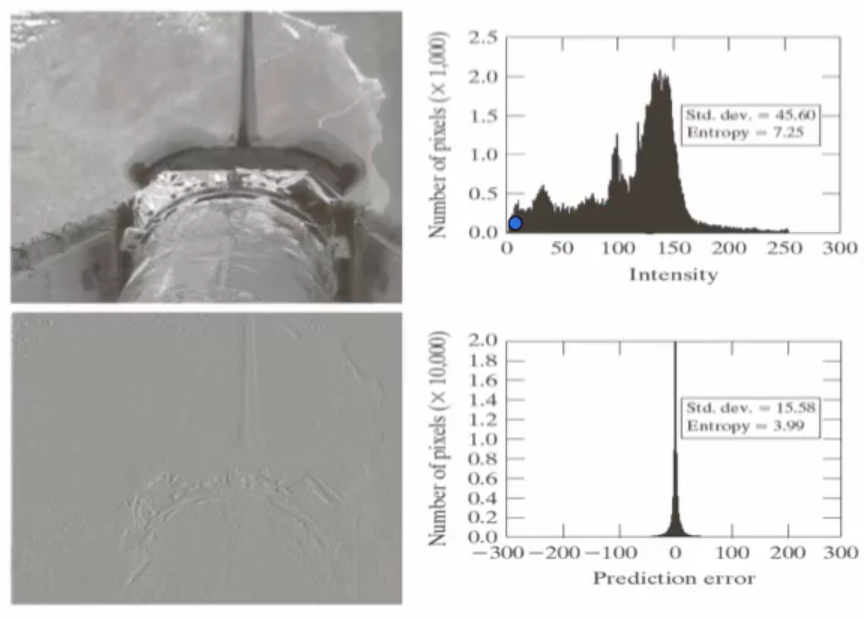
\includegraphics[scale=0.4]{img/predictive_encoding.png}
    \end{center}

\section{Spatial Processing}

  \subsection{Image Enhancement}

    If we have an image that is very dark, we would like to transform it so that we can see it better. More generally, we can take every pixel value $r$ in the image and transform it with a one-dimensional function $T$ to a new value $s$. Two examples are shown below. 
    \begin{enumerate}
        \item The left function shows that moderately dark or moderately light pixels will be pushed to their thresholds, becoming very dark and very light. 
        \item The right function is a thresholding function, pushing every pixel value less than 128 to 0 (black) and all pixel values at least 128 to 255 (white). 
    \end{enumerate}
    \begin{center}
        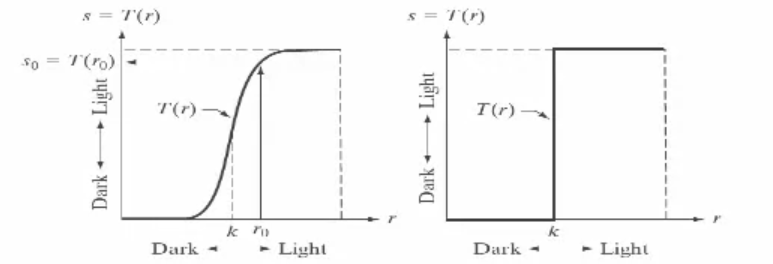
\includegraphics[scale=0.4]{img/point_function.png}
    \end{center}
    In general, we can have the following operations. 
    \begin{center}
        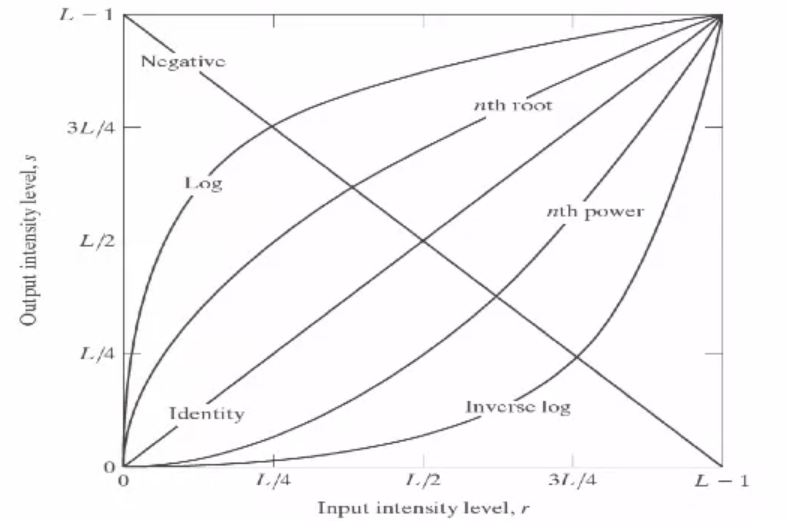
\includegraphics[scale=0.4]{img/point_functions.png}
    \end{center}
    For example, the identity is that $s = t$, but we can have other functions such as $s = c \times \log(t + 1)$, where $c$ is some constant and we have to add $1$ to prevent logarithm of $0$. The inverse function is $s = 255 - t$ and the exponential function is $s = c \cdot t^\gamma$. You can more closely see how the different $\gamma$'s give different functions, and this is called \textbf{gamma correction}. 
    \begin{center}
        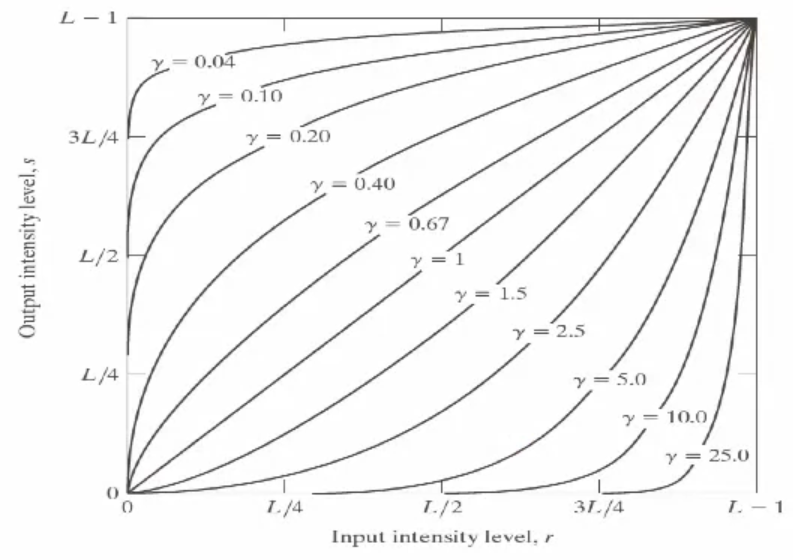
\includegraphics[scale=0.3]{img/gamma_correction.png}
    \end{center}
    This is used in monitors a lot to balance the brightness so that many places do not become dark. 
    \begin{center}
        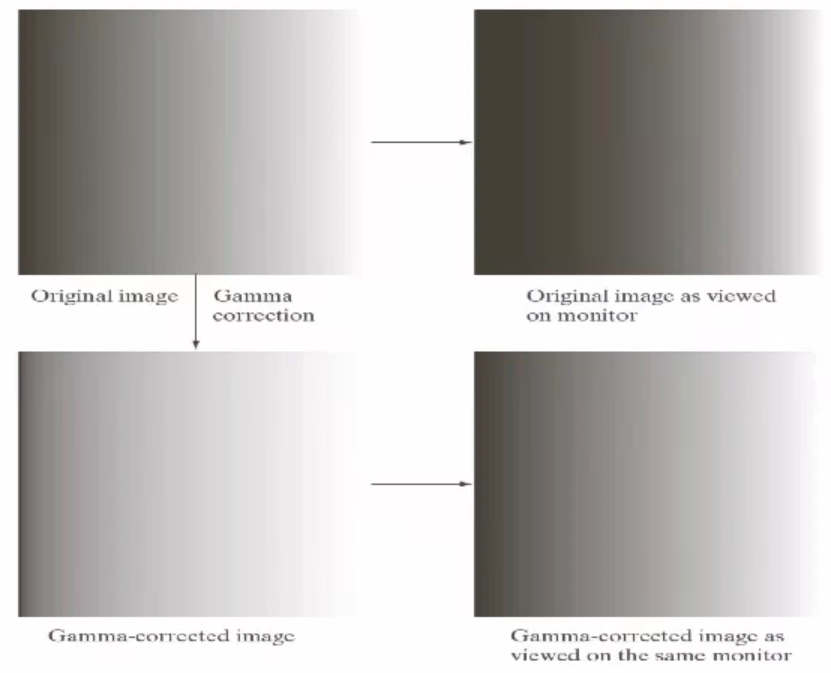
\includegraphics[scale=0.3]{img/gamma_correction2.png}
    \end{center}

    \begin{example}[Contrast Stretching]
    One way we can construct a function is to do \textbf{contrast stretching}, which transforms mid-pixel values and stretches them out, while compressing the extreme pixel values. This results from the top right image to the bottom left image. Then, we can do a thresholding function to further get these contrasts (bottom right). 
    \begin{center}
        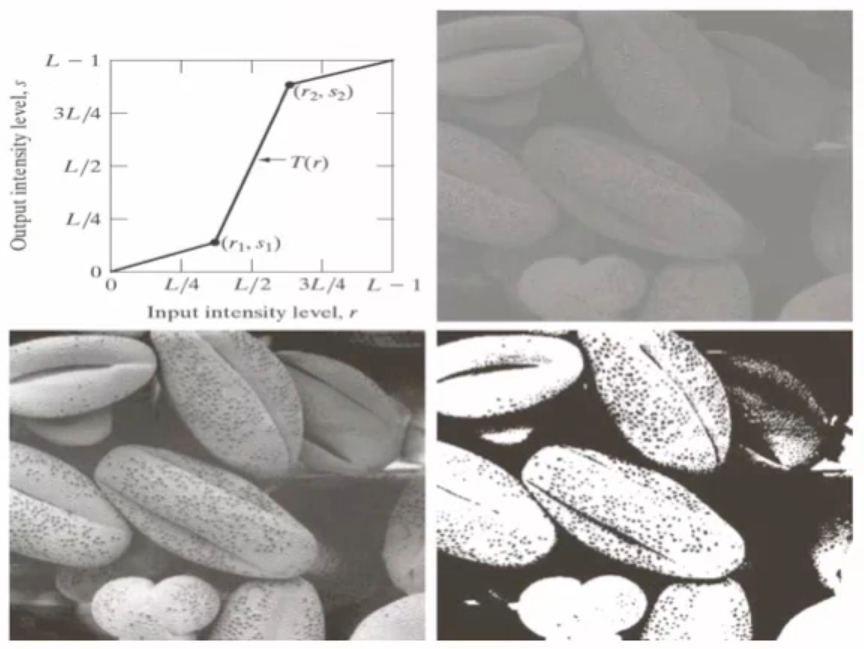
\includegraphics[scale=0.3]{img/contrast_stretching.png}
    \end{center}
    \end{example}

    \begin{example}
    \textbf{Intensity transformations} highlights an intensity range $[A, B]$ and reduces all other intensities to a lower level or preserves them. 
    \begin{center}
        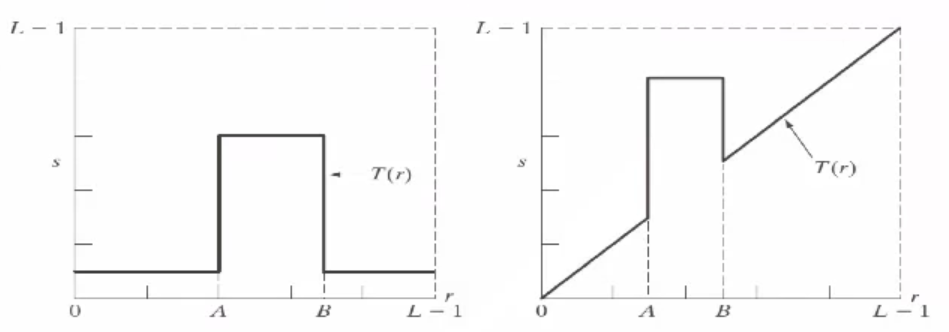
\includegraphics[scale=0.3]{img/intensity_transformations.png}
    \end{center}
    \end{example}

  \subsection{Histogram Equalization and Matching}

    In general, we have 
    \begin{enumerate}
        \item If the image is very dark, the color histogram will be concentrated towards $0$. 
        \item If the image is bright, the color histogram will be concentrated towards $255$. 
        \item If the image is low-contrast, the histogram will just be concentrated somewhere. 
        \item If the image is high-contrast, the histogram will be roughly uniform. 
    \end{enumerate}
    Our goal is to take an arbitrary distribution $R$ over $[L-1]$ and transform it into a uniform distribution $S$. It is well known from probability that if we have a transformation $s = T(r)$ over a discrete state space, then 
    \[\mathbb{P}(S = s) = \mathbb{P}(R = r) \cdot \bigg| \frac{\partial r}{\partial s} \bigg| \]
    Now let us write our transformation as 
    \[s = T(r) = (L - 1) \int_0^r p_R (w) \, dw\]
    That is, if I want to find where I should transform $r$ to, I want to count all the pixel probabilities up until $r$, and normalize it by $L-1$. To prove this, we compute 
    \[\frac{\partial s}{\partial r} = (L-1) \frac{\partial}{\partial r} \int_0^r p_R (w) \,dw = (L-1) \cdot p_R (r)\]
    For single variable functions, $\frac{\partial r}{\partial s} =  1/ \frac{\partial s}{\partial r}$, and so using that and substituting it in gives 
    \[p_S (s) = p_R (r) \frac{1}{(L-1) \, p_R (r)} \frac{1}{L-1}\]
    which is what we want. Note that $T$ will always be monotonic. However, due to us working in discrete spaces, it will not always be perfectly uniform since all pixels with the same value are mapped to the same value. 

    \begin{example}
    Below we have an illustration of histogram equalization of a 3-bit (8 intensity levels) image. The original histogram is on the left, the transform in the middle, and the equalized histogram on the right. 
    \begin{center}
        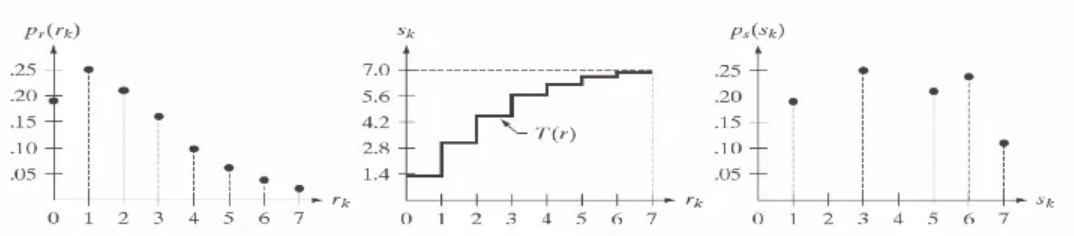
\includegraphics[scale=0.4]{img/hist_equalization.png}
    \end{center}
    \end{example}

    Now \textbf{histogram matching} is a generalization of equalization in the fact that we want to map to any arbitrary distribution $S$, not just uniform, from our original $R$. But we already know how to do this. Given our desired distribution $S$ and our original distribution $R$. We know how to equalize $R$ to a uniform $U$. That is, we know $U = T_1 (R)$. We also can do the same for $U = T_2 (S)$ since $S$ is an arbitrary distribution. Then by taking the inverse of $S$ (disregarding at the moment that it is not invertible in the mathematical sense), we can construct the transformation 
    \[S = (T_2^{-1} \circ T_1) (R)\]
    Now to take care of the inversion problem, say that $R = 7$ maps to $U = 10$, and $S = [15, 20]$ maps to $U = 10$ also. Then $R = 7$ can map to any $S \in [15, 20]$, and mainly it is the smallest one: $15$. 

    Finally, sometimes we want higher contrast in different regions of the image, so we can split the image into different sections and do histogram equalization on each section, improving contrast in every region of the image. 

  \subsection{Local Neighborhood Operations}

    Now a convolution is described by a \textbf{kernel}, also called a \textbf{filter}, which is simply a $K \times K$ matrix. It does not have to be square but is conventionally so. It goes through a grayscale image at every point and compute the dot product of the kernel with the overlapping portion of the image, creating a new pixel. This can be shown in Figure \ref{fig:convolution1}. 

    \begin{figure}
    \centering
    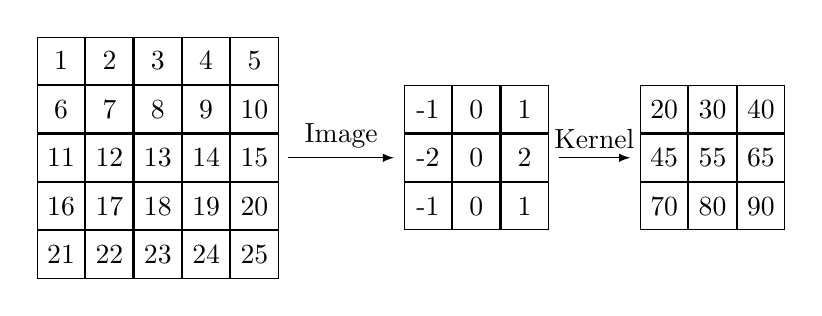
\begin{tikzpicture}[>=latex]

    % Image
    \matrix[matrix of nodes, nodes={draw, minimum size=0.6cm, anchor=center}] (image) {
        1 & 2 & 3 & 4 & 5 \\
        6 & 7 & 8 & 9 & 10 \\
        11 & 12 & 13 & 14 & 15 \\
        16 & 17 & 18 & 19 & 20 \\
        21 & 22 & 23 & 24 & 25 \\
    };

    % Kernel
    \matrix[matrix of nodes, nodes={draw, minimum size=0.6cm, anchor=center}, right=3cm] (kernel) {
        -1 & 0 & 1 \\
        -2 & 0 & 2 \\
        -1 & 0 & 1 \\
    };

    % Convolution result
    \matrix[matrix of nodes, nodes={draw, minimum size=0.6cm, anchor=center}, right=6cm] (result) {
        20 & 30 & 40 \\
        45 & 55 & 65 \\
        70 & 80 & 90 \\
    };

    % Arrows
    \draw[->] (image) -- node[midway, above] {Image} (kernel);
    \draw[->] (kernel) -- node[midway, above] {Kernel} (result);

    \end{tikzpicture}
    \caption{Convolution using a kernel on an image.}
    \label{fig:convolution1}
    \end{figure}

    Now if this was a color image, then the $K \times K$ kernel $\mathcal{K}$ would dot over all 3 layers, without changing over all 3 layers. This is equivalent to applying the kernel over all 3 channels separately, and then combining them together into one. Another thing to note is that the output image of a kernel would be slightly smaller than the input image, since the kernel cannot go over the edge. However, there are padding schemes to preserve the original dimensions. 

    Note that the kernel matrix may have the property that all of its entries sum to $1$, meaning that on average, the expected value of the brightness of each pixel will be $0$, and the values will be left unchanged on average. However, this is not a requirement. 

    \begin{example}[Mean Blur, Gaussian Blur]
    The mean and Gaussian blur is defined with kernels that are distributed uniformly and normally across the entire matrix. You can see how this would blur an image since for every pixel, we take the weighted average over all of its surrounding pixels. 

    \[\text{mean} = \frac{1}{25} \begin{bmatrix} 1 & 1 & 1 & 1 & 1 \\ 1 & 1 & 1 & 1 & 1 \\ 1 & 1 & 1 & 1 & 1 \\ 1 & 1 & 1 & 1 & 1 \\ 1 & 1 & 1 & 1 & 1 \end{bmatrix}, \;\;\;\;\; \text{Gaussian} = \frac{1}{273} \begin{bmatrix} 1 & 4 & 7 & 4 & 1 \\ 4 & 16 & 26 & 16 & 4 \\ 7 & 26 & 41 & 26 & 7 \\ 4 & 16 & 26 & 16 & 4 \\ 1 & 4 & 7 & 4 & 1 \end{bmatrix}\]

    On a large scale, there really aren't any discernable differences, as seen in the figure but the Guassian blur is known to be a more realistic representation of how humans receive blur. 
    \begin{figure}[H]
      \centering
      \begin{subfigure}[b]{0.32\textwidth}
      \centering
          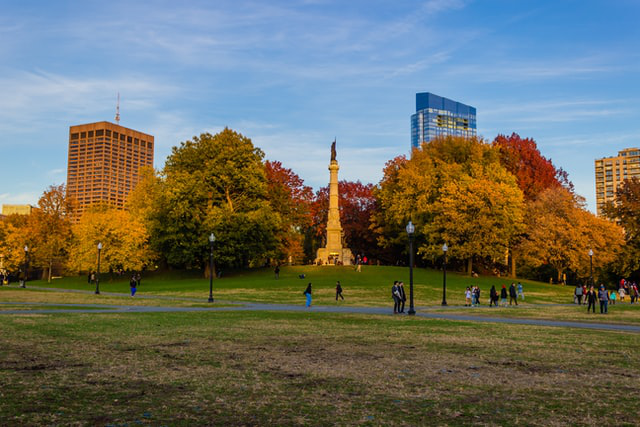
\includegraphics[width=\textwidth]{img/Park_Full.png}
          \caption{Original image. }
          \label{fig:Park_full}
      \end{subfigure}
      \begin{subfigure}[b]{0.32\textwidth}
      \centering
          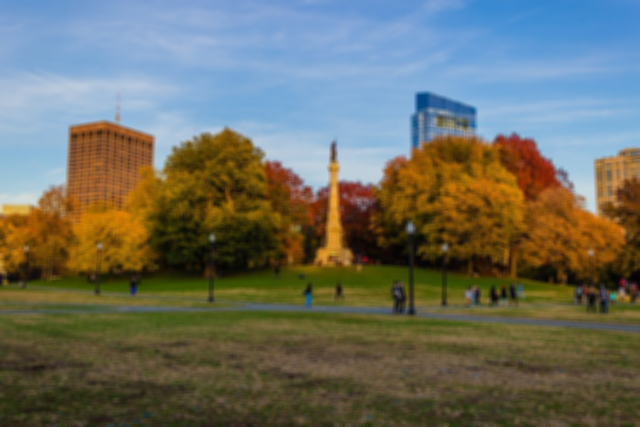
\includegraphics[width=\textwidth]{img/Mean_Blur.png}
          \caption{$5 \times 5$ mean blur applied. }
          \label{fig:Mean_blur}
      \end{subfigure}
      \begin{subfigure}[b]{0.32\textwidth}
      \centering
          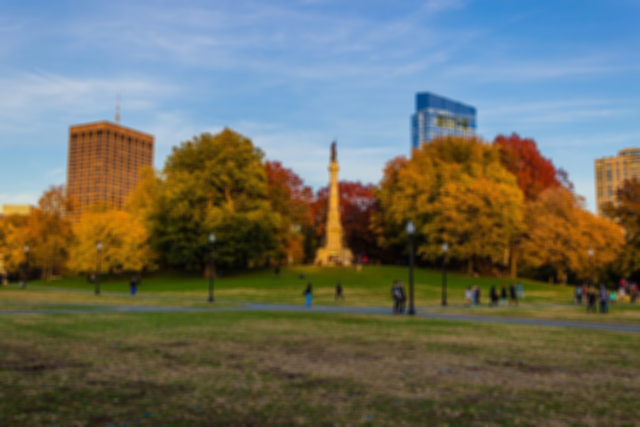
\includegraphics[width=\textwidth]{img/Gaussian_Blur.png}
          \caption{$5 \times 5$ Gaussian blur applied. }
          \label{fig:gaussian_blur}
      \end{subfigure}
      
      \caption{Comparison of blurring kernels on image. }
      \label{fig:blur}
    \end{figure}
    \end{example}

    Note that given an image $f(x, y)$, the mean blur simply picks the new pixel value of $(x, y)$ as the one that minimizes the least square error 
    \[\argmin_k \sum_{(x, y) \in M} \big( f(x, y) - k \big)^2\]
    which happens to be the average of the pixel values in the kernel region $M$. The Gaussian blurring can be thought of as a convolution 
    \[f(x, y, \sigma) = f(x, y) \ast N(0, \sigma^2)\]
    which corresponds to the heat flow equation defined 
    \[\frac{\partial f}{\partial t} = \Delta f = \frac{\partial^2 f}{\partial x^2} + \frac{\partial^2 f}{\partial y^2}\]

    \begin{example}[Median Filter]
    The median filter acts like the mean filter but it doesn't have as much blurring. This is great when we need to reduce noise but still want some contrast between edges. 
    \begin{center}
        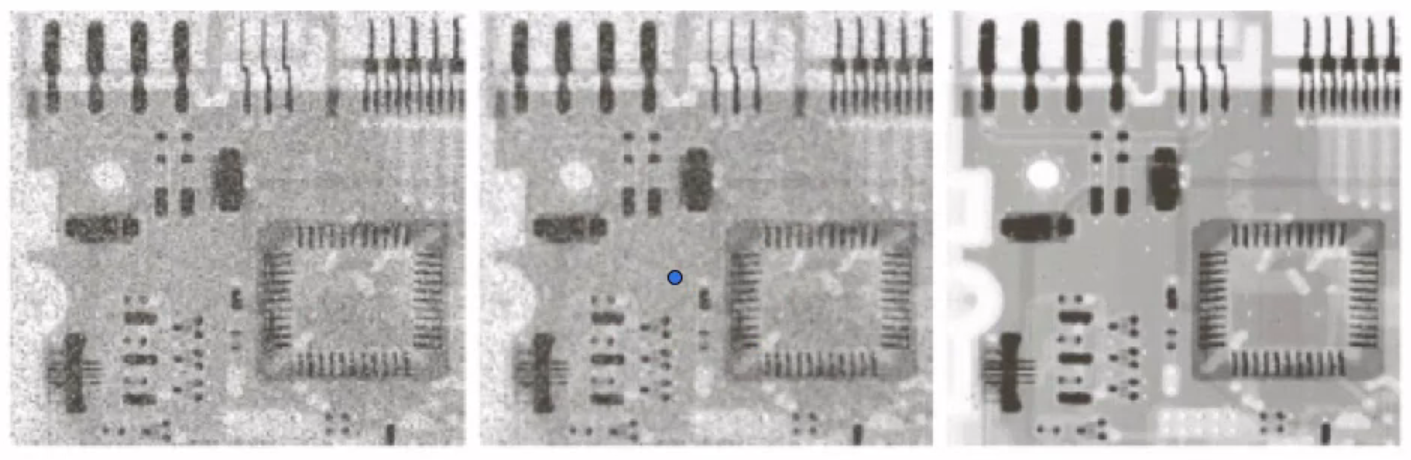
\includegraphics[scale=0.25]{img/median_filter.png}
    \end{center}
    It turns out that the median filter is the argmin of not the squared error, but the absolute value error 
    \[\argmin_k \sum_{(x, y) \in M} \big| f(x, y) - k \big|\]
    \end{example}

  \subsection{Non Local Means}

    The point of non local averaging is to take away the limitations of averaging over local neighborhoods, but rather through many sections that may be far away from each other, yet still looks the same. For examples, there are many sections in the image that are not next to each other, but are very similar. 
    \begin{center}
        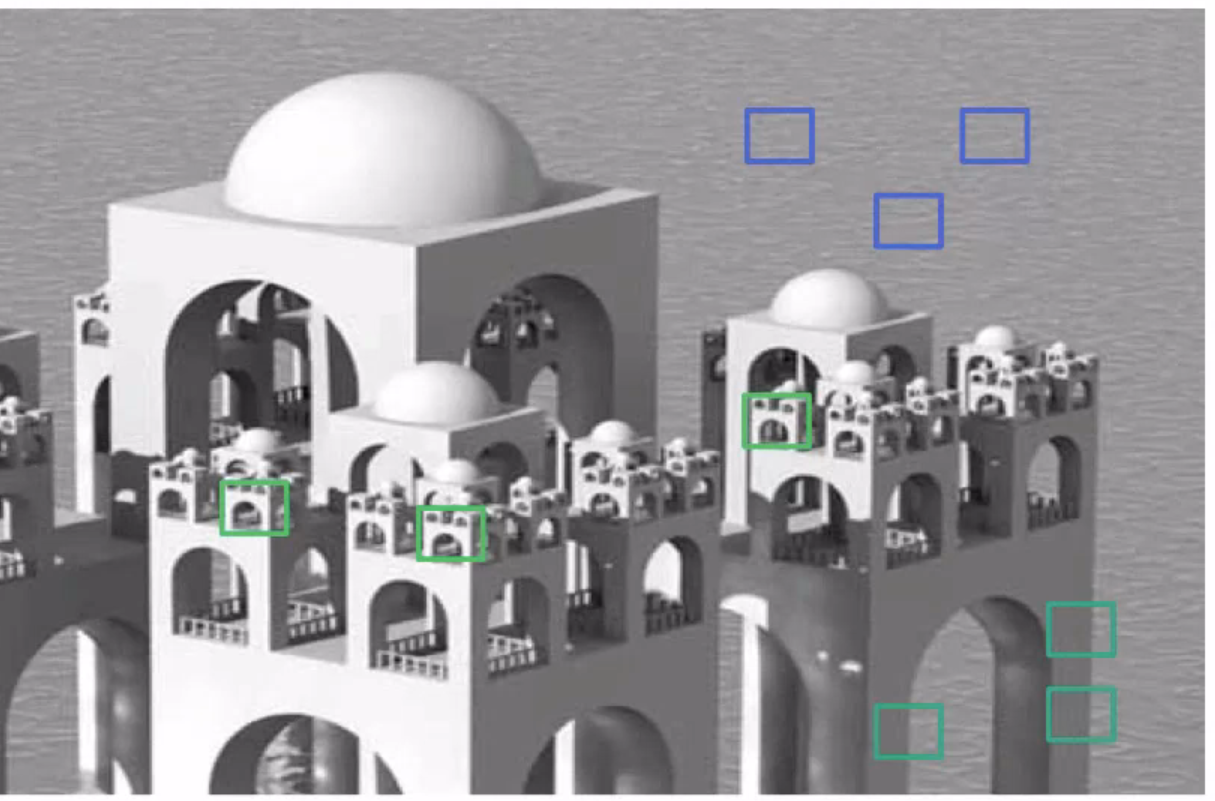
\includegraphics[scale=0.2]{img/nonlocal_average.png}
    \end{center}
    Now it turns out that if we have a pixel value $p_0$ and observe it many times, we expect it to be different according to some noise $\epsilon$, which is a random variable. 
    \begin{align*}
        p_1 & = p_0 + \epsilon \\ 
        p_2 & = p_0 + \epsilon \\ 
        \ldots & = \ldots \\ 
        p_N & = p_0 + \epsilon
    \end{align*}
    But it turns out that if we observe $N$ variations of these, by averaging them out the noise reduces by a factor of $N^2$. We still haven't specified two things: 
    \begin{enumerate}
        \item How to look for neighborhoods that are similar to each other. 
        \item Once we have these neighborhoods, how do we average them? Or do some other operation? 
    \end{enumerate}

  \subsection{Laplacian and Unsharp Masking}

    When we have a, say 1-dimensional image, the first derivative of the pixel intensities can be approximated by the finite differences between adjacent values. 
    \[\frac{\partial f}{\partial x} = f(x + 1) - f(x)\]
    We can define this similarly for the second derivative 
    \[\frac{\partial^2 f}{\partial x^2} = f(x + 1) + f(x - 1) - 2 f(x)\]
    Note that the coefficients are $1, -2, 1$. This second derivative gives us information on the curvature of the pixel intensities. That is, if the curvature is high, then there may be an abrupt change intensity of the pixel values. Extending this to the two-dimensional image gives us the Laplacian of $f$: 
    \[\Delta f = \frac{\partial^2 f}{\partial x^2} + \frac{\partial^2 f}{\partial y^2}\]
    resulting in a kernel that looks like 
    \[\begin{bmatrix} 0 & 1 & 0 \\ 1 & -4 & 1 \\ 0 & 1 & 0 \end{bmatrix}\]
    Which is actually the kernel that is used to sharpen images, and the diagram below gives an idea on how it is done. 
    \begin{center}
        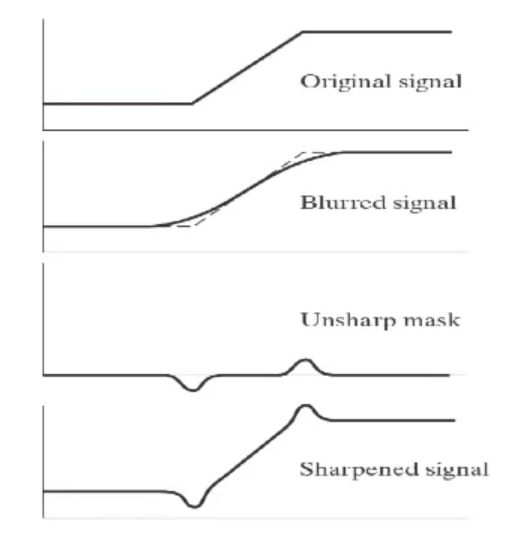
\includegraphics[scale=0.4]{img/sharpen.png}
    \end{center}
    Given an image $I$ and the transformation $T$, we can take $T(I)$ and add it to $I$ to generate a sharpened image. 
    \begin{center}
        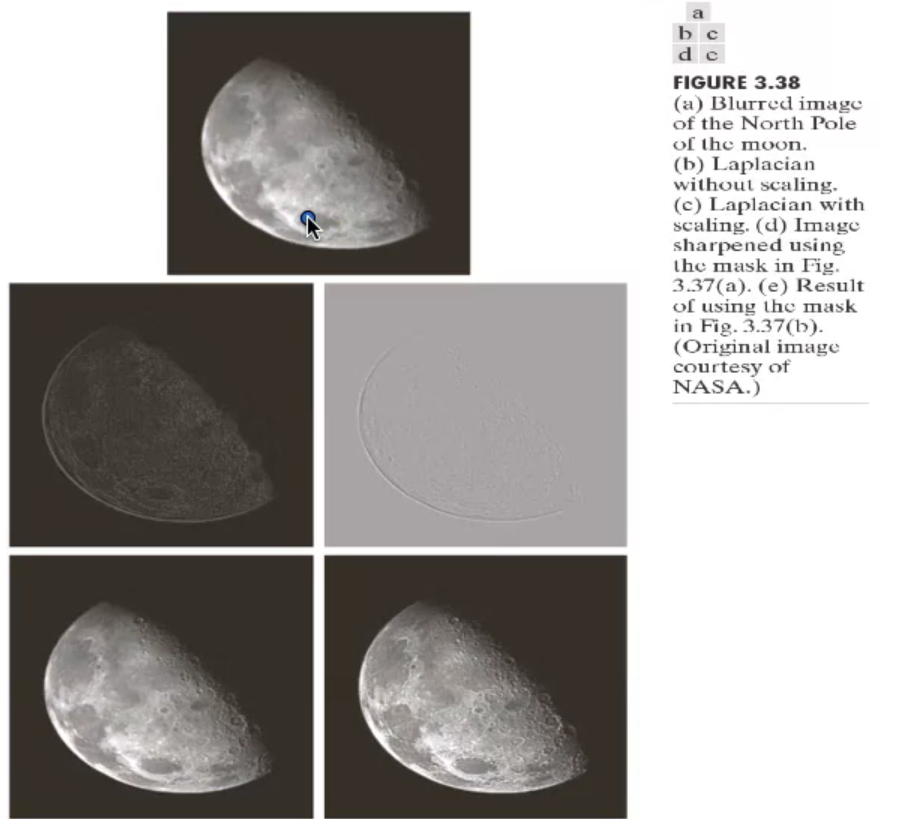
\includegraphics[scale=0.4]{img/laplacian_unsharpen.png}
    \end{center}

\section{Image Restoration}

    When we take an image, there may be some source of degradation of it in the form of motion blur, along with some noise. We can model the image as $f(x, y)$, which can be convolved using the degradation function $H$, and finally added with some noise $\eta$ (usually assumed, but not always additive and could be multiplicative), giving us 
    \[g(x, y) = \big[ f(x, y) \ast H(x, y) \big] + \eta(x, y)\]
    One of the effects of multiplicative noise is that the amount of noise is dependent on the signal itself. If you do have multiplicative noise, then we can just take the logarithm of the equation to get additive noise in the log scale, and so the additive noise model is still applicable, albeit with some limitations. We would like to restore this image to some approximation $\hat{f}(x, y) \approx f(x, y)$. 
    \begin{center}
        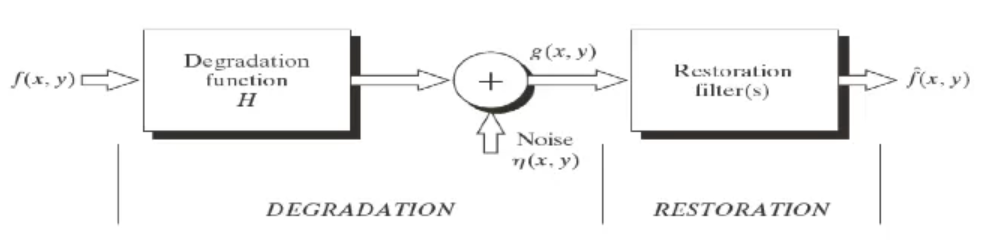
\includegraphics[scale=0.3]{img/degradation_restoration.png}
    \end{center}

  \subsection{Types of Noise}

    The additive noise $\eta$ can be modeled by different probability distributions: 
    \begin{enumerate}
      \item Gaussian noise is used a lot due to its nice mathematical properties and approximations, but there aren't many natural processes that actual produce Gaussian noise. 
      \[p(x) = \frac{1}{\sqrt{2 \pi} \sigma} e^{-\frac{(x - \mu)^2}{2 \sigma^2}} \]

      \item The Raleigh distribution is defined 
      \[p(x) = \begin{cases} \frac{2}{b} (x - a) e^{-(x - a)^2 / b} & \text{ if } x \geq a \\ 0 & \text{ if } z \leq a \end{cases}\]
      which has the mean and variance 
      \[\mathbb{E}[X] = a + \frac{\sqrt{\pi b}}{2} \text{ and } \mathrm{Var}[X] = \frac{b (4 - \pi)}{4}\]

      \item The exponential noise 
      \[p(x) = \begin{cases} \lambda e^{-\lambda x} & \text{ if } x \geq 0 \\ 0 & \text{ if } x < 0 \end{cases}\]
      with 
      \[\mathbb{E}[X] = \frac{1}{\lambda} \text{ and } \mathrm{Var}[X] = \frac{1}{\lambda^2}\]

      \item The uniform noise 
      \item The impulse noise, also called the salt and pepper noise, is a Bernoulli random variable, since we are either changing the pixel value to either white (salt) or black (pepper). It doesn't act on every pixel, but rather a very small random subset of pixels in the image. It is a good model for when you have a broken sensor that doesn't collect light at a certain point in the lens. 
    \end{enumerate}

    The following shows the distributions. 
    \begin{center}
        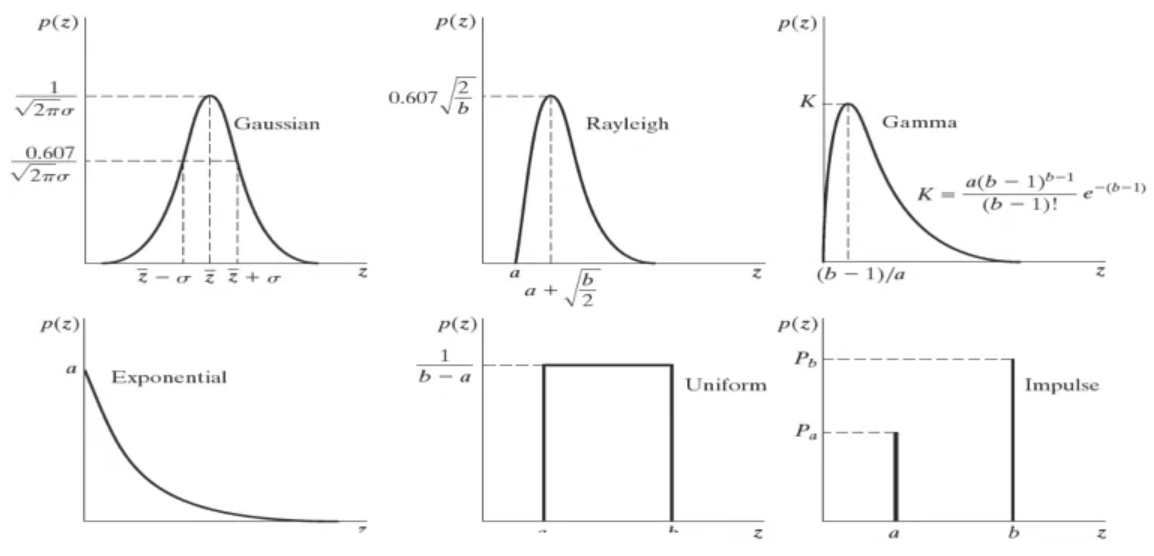
\includegraphics[scale=0.3]{img/noise_distributions.png}
    \end{center}
    and given an image of 3 pixel values (say, white, grey, and black), the following color histograms are produced after adding Gaussian, Rayleigh, and Gamma noise. 
    \begin{center}
        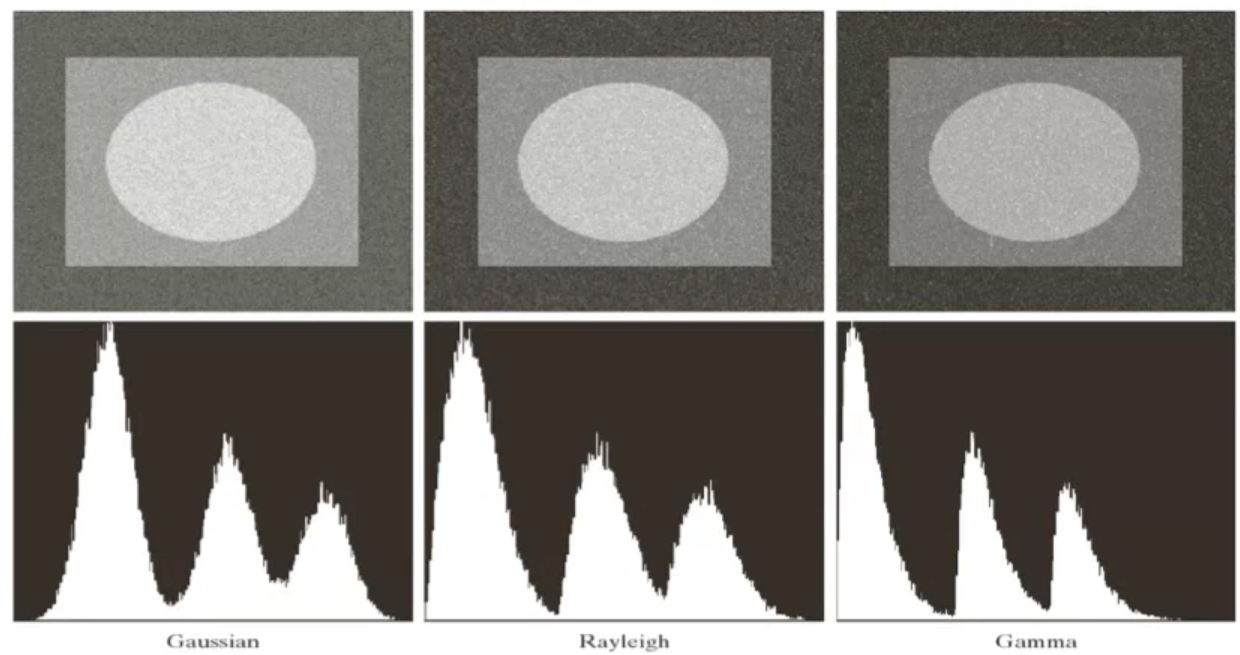
\includegraphics[scale=0.3]{img/noise_histograms.png}
    \end{center}

  \subsection{Estimating Noise}

    Now, given a section of an image with a constant pixel value (as shown in the grey region in the blue box), we assume that it will have some intrinsic noise $\eta$ on top of it. The thing is we have no idea what the actual distribution of $\eta$ is. However, we do have samples from this region, and therefore, we can use a maximum likelihood estimate (MLE) for a class of pre-given distributions. 
    \begin{center}
        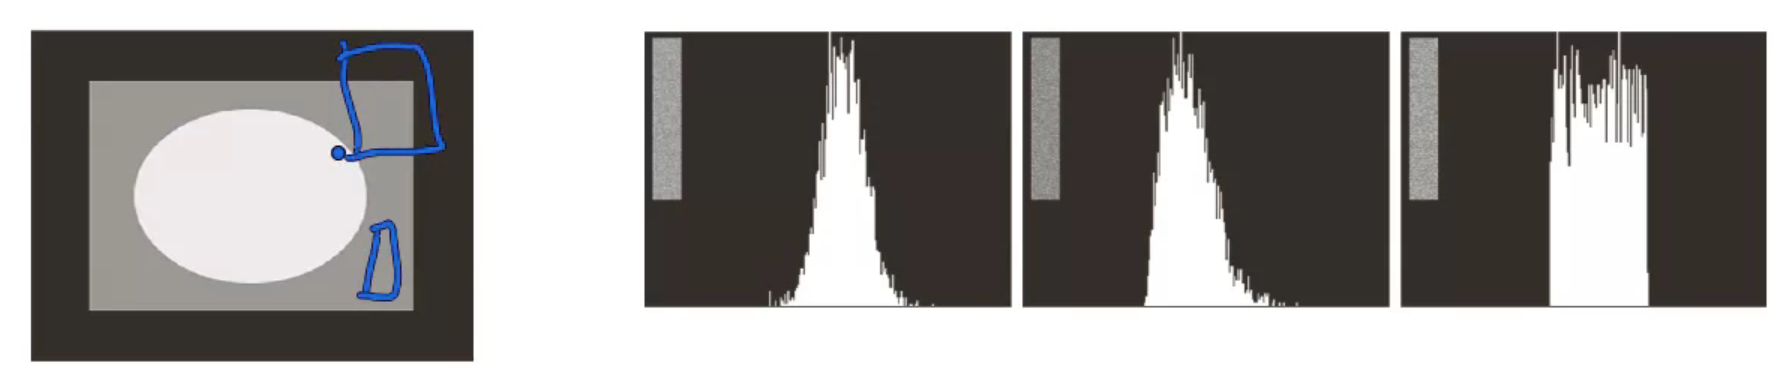
\includegraphics[scale=0.2]{img/hist_estimate.png}
    \end{center}
    For the picture above, taking samples from the uniform grey region above will give some distribution as a histogram, and depending on the shape of it (more mathematically, by maximizing the likelihood), we can approximate the $\eta$. Now if we have regions that aren't guaranteed to be coming from one pixel value, such as the larger blue box above, then it becomes harder since there is an extra layer of uncertainty. We can split this into smaller regions and assume that a small region maintains a relatively constant pixel value, but splitting it too much will lead to smaller samples. 

    Once we can estimate the best distribution that the noise came from, we can use the appropriate filtering methods. 
    \begin{enumerate}
        \item To remove uniform and Gaussian noise, we use the average filter (local or non local means). 
        \item To remove salt and pepper noise, we use the median filter. 
    \end{enumerate}

  \subsection{Estimating Degradation Function}

    Now given the degraded image 
    \[g(x, y) = f(x, y) \ast h(x, y) + \eta(x, y)\]
    we have learned how to estimate the $\eta$, but estimating $h$ is much harder. In a general sense, we can take the Fourier transform of both sides to convert the convolution to a product in a different domain, and simply divide to get $F$. 
    \[G(u, v) = F(u, v) \cdot H(u, v) \implies F(u, v) = \frac{G(u, v)}{H(u, v)}\]
    In fact, due to the commutativity of the convolution operator, it isn't even clear whether $f$ is the original image of $h$. Additionally, it is very unstable since the Gaussian may be close to $0$, and this isn't a very good way to filter. 

    \begin{example}[Gaussian Blurring]
    The blurring degradation effect can be observed by the convolution kernel $h$ being a Gaussian function. 
    \begin{center}
        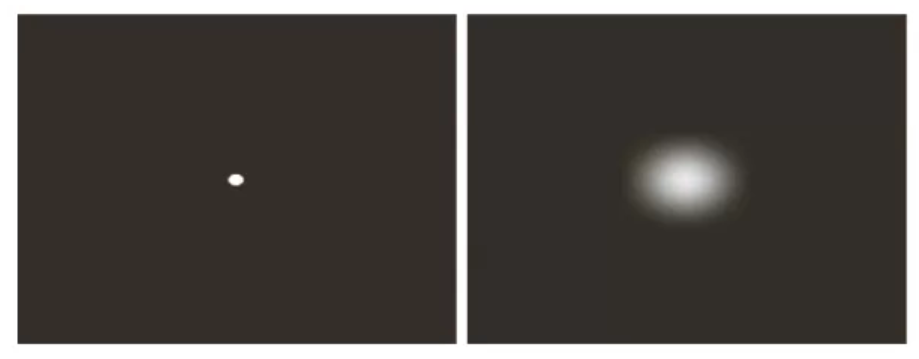
\includegraphics[scale=0.3 ]{img/delta_blurring.png}
    \end{center}
    In fact, when we have a point of light, which is basically a delta function $\delta$ and put the Gaussian filter $G \sim N(0, \sigma^2)$ on it, we know that $G = \delta \ast G$, so use can actually use this calibrate cameras. The camera can artificially create a point of light, and then estimate the variance of the Gaussian that it actually detects, which estimates the blur. 
    \end{example}

    \begin{example}[Motion Blurring]
    When we move the camera while taking a picture, the camera integrates the light that comes into the sensor, and therefore we get motion blurring. Mathematically, the actual image is 
    \[g(x, y) = \int_0^T f\big( x - x(t), y - y(t)\big) \,dt\]
    \begin{center}
        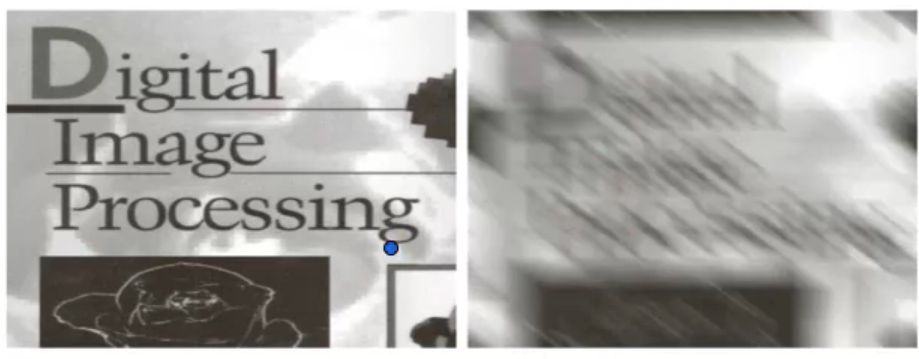
\includegraphics[scale=0.3]{img/motion_blurring.png}
    \end{center}
    Clearly, getting the original function $f$ from an integrated version of it is overdeterministic. That's like saying solve $x + y = 5$ for $(x, y)$, which has an infinite number of solutions. But there are more advanced methods. 
    \end{example}

  \subsection{Weiner Filtering}

    Now let's talk about the restoration filter. Right now, given the original image, degraded into $g$, noise added, and then restored into $\hat{f}$, i.e. 
    \[f \mapsto g = f \ast h \mapsto g + \eta \mapsto \hat{f}\]
    we can compute the error between our restored image and the original with the MSE 
    \[e^2 = \mathbb{E}[ ( f(x, y) - \hat{f}(x, y))^2]\]
    Now, what we want to do is do a Fourier transform on $\hat{f}$, and working in the Fourier domain and minimizing the $e^2$ (by taking the derivative and setting it to $0$) gives 
    \[\hat{F}(u, v) = \underbrace{\frac{H^\ast (u, v)}{H^2 (u, v) + S_\eta / S_f}}_{\text{Weiner Filter}} G(u, v)\]
    Where $H^\ast$ is the complex conjugate of the Fourier transform of the original $h$. To compare the filters, we can see that the top left is $f$, the top right is the degraded observation $g$, the bottom left is the inverse filter $G/H$ (followed by the inverse transform), and the bottom right is the Weiner filter $H^\ast / (H^2 + K)$. 
    \begin{center}
        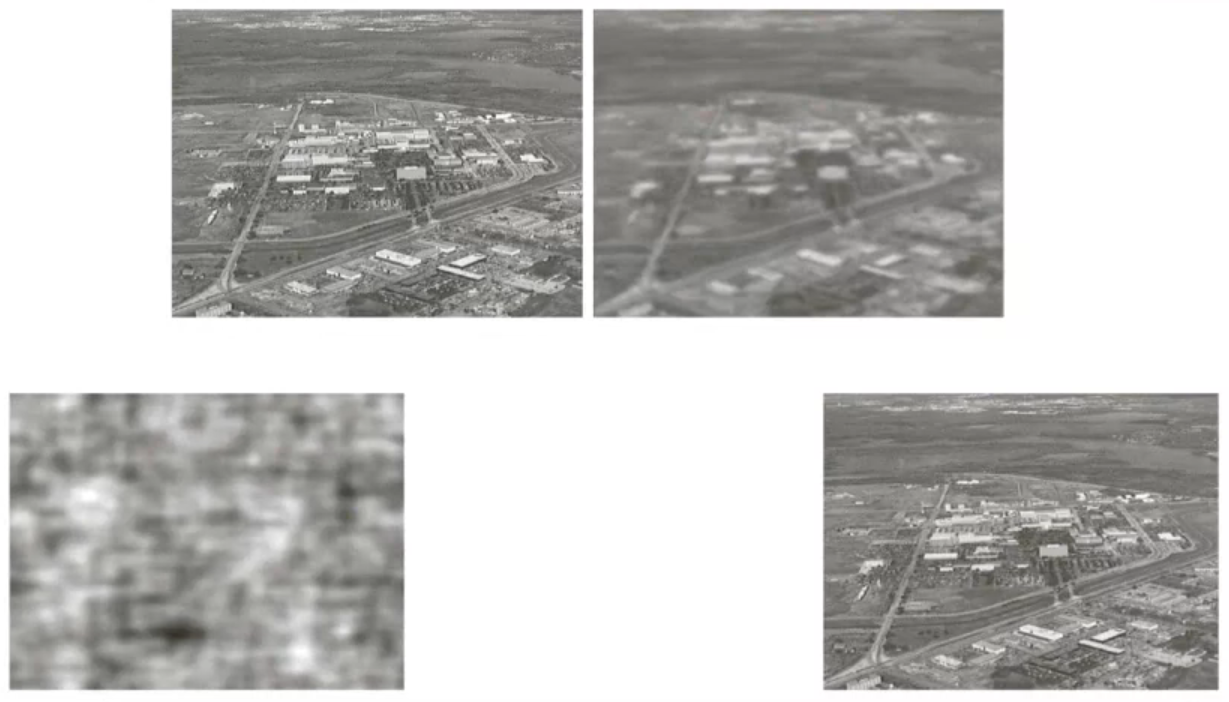
\includegraphics[scale=0.3]{img/filter_comparison.png}
    \end{center}

\section{Image Segmentation}

    The purpose of image segmentation is to identify certain objects and isolate them by drawing boundaries around them. This can be done by detecting edges with gradients, as we can do with the flower below, but this may not always be the case, as with the ball on the right. 
    \begin{center}
        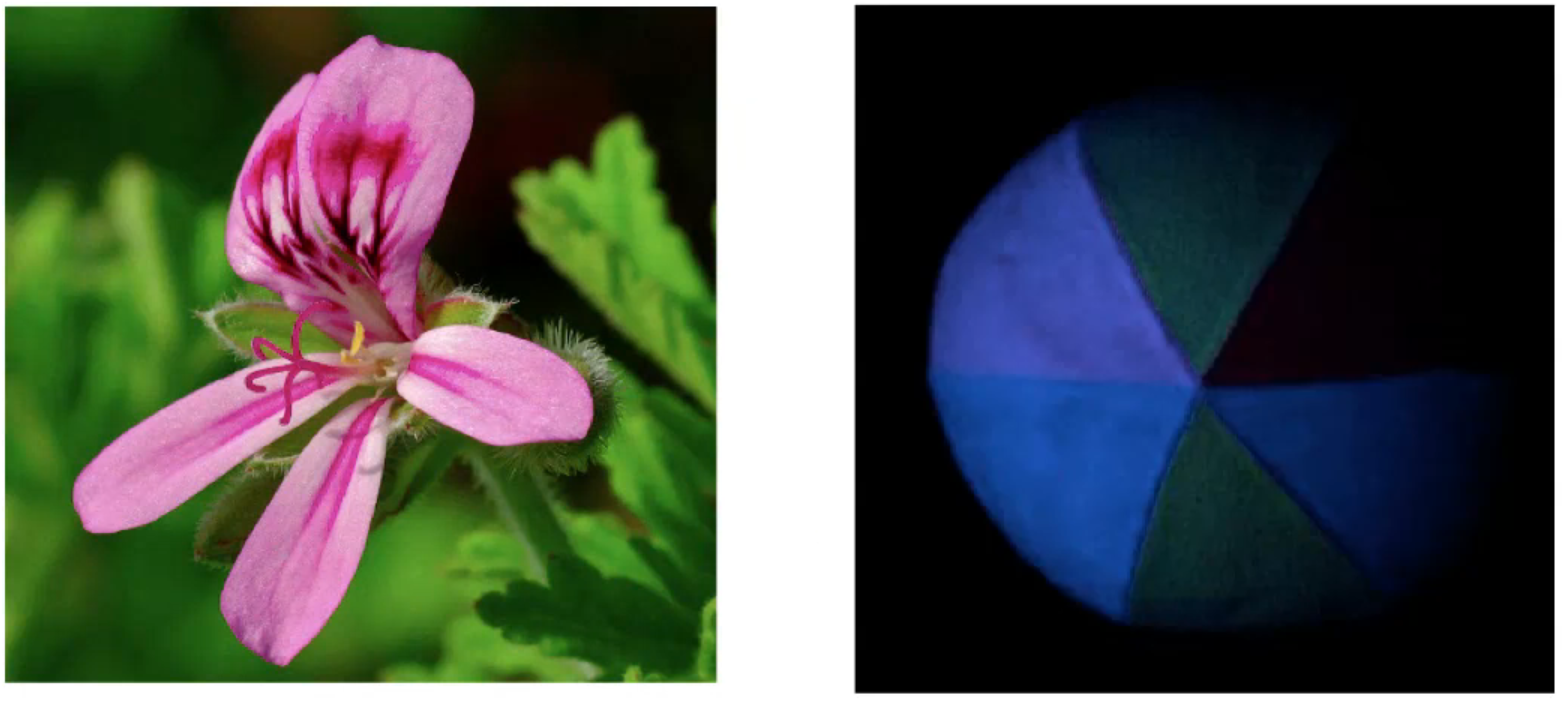
\includegraphics[scale=0.2]{img/segmengation_example.png}
    \end{center}

  \subsection{Hough Transform}

    The simplest shapes to detect are lines, which we will start off with first. A line can be parameterized with two parameters: $\rho$, the distance between the line and the origin (perpendicular to the line), and $\theta$, which is the angle that the segment connecting the origin to the line makes with the x-axis. It is the set of all $(x, y)$ that satisfies 
    \[\rho = x \cos{\theta} + y \sin{\theta}\]
    \begin{center}
        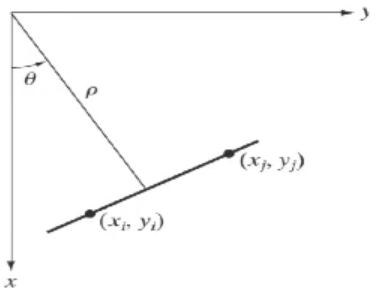
\includegraphics[scale=0.4]{img/line.png}
    \end{center}
    Now the set of all possible lines lives within the $(\rho, \theta)$ space, and is two dimensional. Now fix a point $(x_0, y_0)$ in the XY plane. Then, the set of lines that pass through $(x_0, y_0)$ forms a one-dimensional curve in $\mathbb{R}^2_{(\rho, \theta)}$. Now take another point $(x_1, y_1)$ and do the same, forming another 1-dimensional curve. It turns out that these curves are sinusoidal, and they will have an intersection somewhere, which is precisely the line that passes through $(x_0, y_0)$ and $(x_1, y_1)$. Therefore, by drawing these curves, we can identify the line that passes through these two points. since we're working with computer systems, this is all discretized and we have a certain max and min value for each $(\rho, \theta)$. 
    \begin{center}
        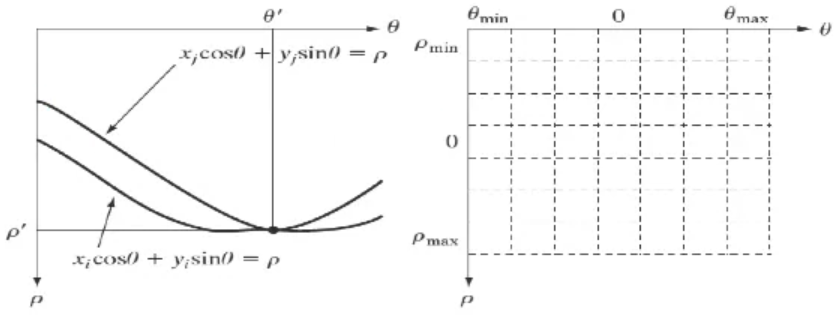
\includegraphics[scale=0.4]{img/rho_theta.png}
    \end{center}
    Now the Hough transform first does edge detection on the image, which gives us a collection of points $\{ (x_i, y_i)\}$, and for each point, we draw the sinusoidal curve of all possible lines going through that point. This set of all parameterized curves is called the accumulator. We can see an example below, where we first do edge detection (top right) on the original image (top left), and then we create the accumulator. We then take the point $(\rho^\ast, \theta^\ast)$ or the set of points that passes a certain threshold on the number of votes. 
    \begin{center}
        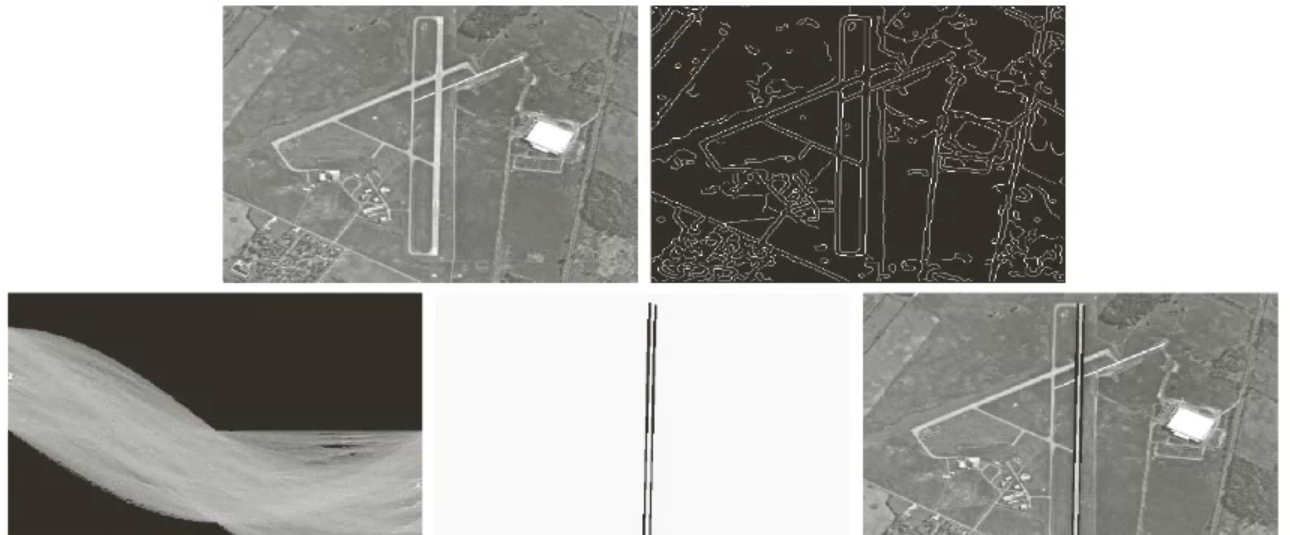
\includegraphics[scale=0.3]{img/accumulator.png}
    \end{center}

    To detect circles, note that a circle can be parameterized by 3 scalars: $x_0, y_0, r$, as 
    \[(x - x_0)^2 + (y - y_0)^2 = r^2\]
    and so for each point, the accumulator will be in a 3-dimensional space. We accumulate and identify the circles with the maximal accumulated values. 
    \begin{center}
        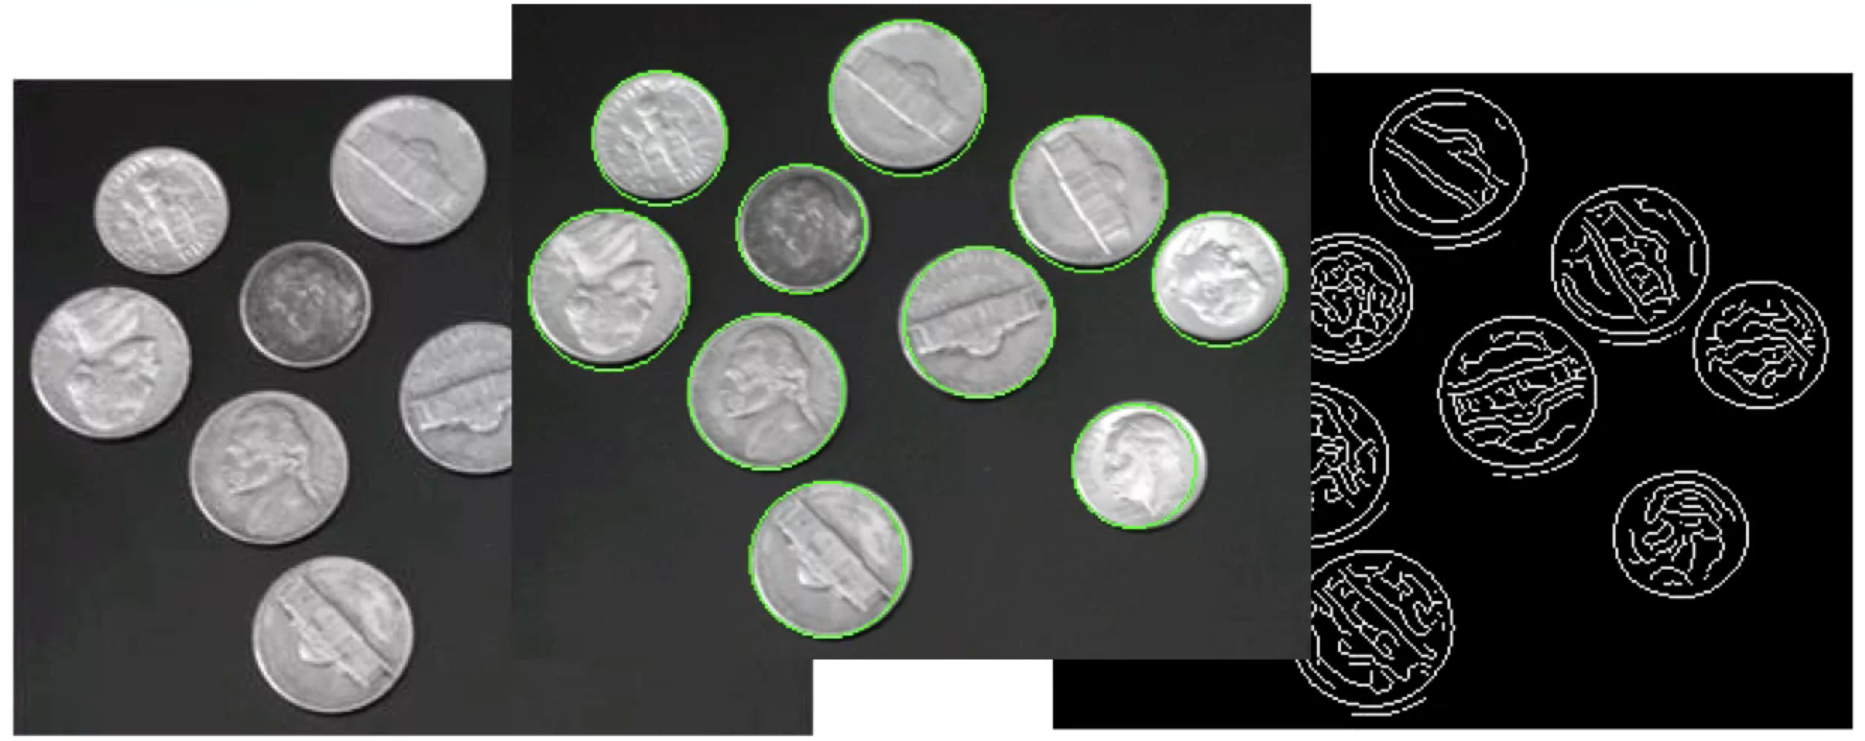
\includegraphics[scale=0.2]{img/circle_accum.png}
    \end{center}

  \subsection{Otsu's Segmentation}

    Let's say we have an image that consists of just two pixel values. Then, we can simply set a thresholding function that maps one value to $255$ and the other to $0$, which is basically segmentation. If there is noise, then we have a bimodal color distribution, and Otsu's method automatically identifies the threshold value between $0$ and $255$ that we should threshold on. It works naturally well with the first two images, but if there is a lot of noise (as in the 3rd image), then we can simply denoise it with the processes described previously to get a bimodal distribution, and then perform Otsu's after. 
    \begin{center}
        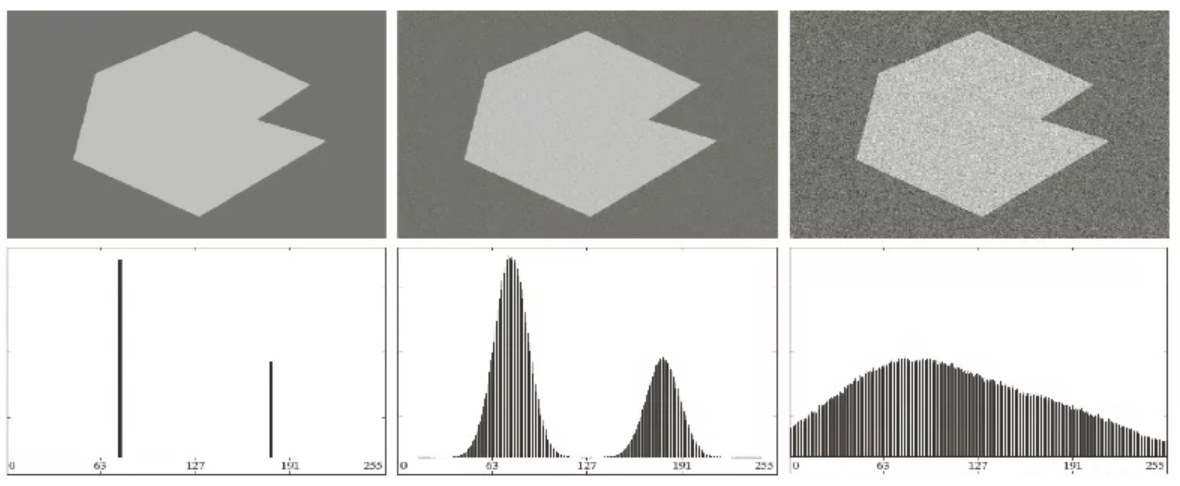
\includegraphics[scale=0.3]{img/otsu1.png}
    \end{center}
    Otsu's segmentation assumes that we have 2 classes, and we have to minimize the weighted within-class variance. Intuitively, we want to determine a threshold such that all the values to the left are in one distribution and all to the right are in another, and taking the weighted sum of the variances should be minimized. Since the variance increases quadratically, we wouldn't want far-tailed distributions. 
    \begin{enumerate}
        \item First we normalize the histogram so that for $i \in [255]$, $P(i)$ is the probability of a random pixel being color $i$. 
        \item Then for a given $t$, we set 
        \[q_1 (t) = \sum_{i=1}^t P(i) \text{ and } q_2 (t) = \sum_{i=t+1}^{255} P(i)\]
        \item Then we calculate the mean and variance of these distributions. 
        \begin{align*}
            \mu_1 (t) & = \frac{1}{q_1 (t)} \sum_{i=1}^t i P(i) \\
            \mu_2 (t) & = \frac{1}{q_2 (t)} \sum_{i=t+1}^{255} i P(i) \\
            \sigma_1^2 (t) & = \frac{1}{q_1 (t)} \sum_{i=1}^t [ i - \mu_1 (t) ]^2 P(i) \\
            \sigma_2^2 (t) & = \frac{1}{q_2 (t)} \sum_{i=t+1}^{255} [ i - \mu_1 (t) ]^2 P(i) 
        \end{align*}
        \item Then minimize 
        \[\sigma_w^2 (t) = q_1 (t) \sigma_1^2 (t) + q_2 (t) \sigma_2^2 (t)\]
    \end{enumerate}
    We can minimize the final term by brute force, i.e. checking for all $t \in [255]$, but with a bit of algebra, we can see that the total variance of the image can be decomposed to 
    \[\sigma^2 = \sigma_w^2 (t) + q_1(t) [1 - q_1(t)][\mu_1 (t) - \mu_2(t)]^2\]
    and now the problem reduces to maximizing $q_1(t) [1 - q_1(t)][\mu_1 (t) - \mu_2(t)]^2$, which is much easier to compute and can even be computed in a recursive fashion. 

    Even if you have an image that is corrupted by a nonuniform background (and can lead to non-bimodal histograms), performing Otsu's algorithm on the whole image can lead to certain objects being blacked out, as shown below. To fix this, uou can do Otsu's algorithm on subblocks of the image or through moving windows, which minimizes the variance of the background. 
    \begin{center}
        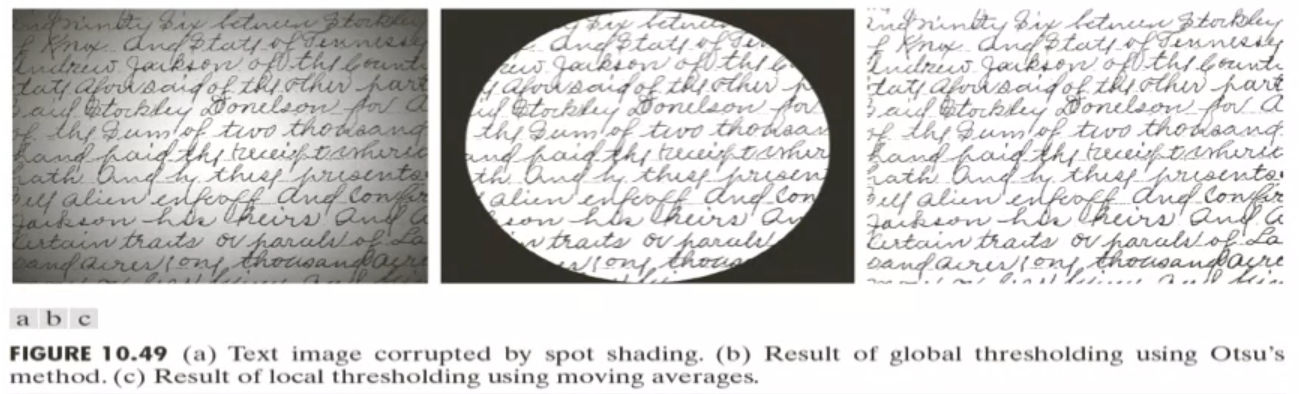
\includegraphics[scale=0.3]{img/otsu2.png}
    \end{center}

  \subsection{Interactive Image Segmentation}

    Interactive image segmentation allows the user to draw line segments that separate the foreground and the background. The first step is to take the pixels across the foreground and background lines and compute its histograms. Then, by going through every other pixel in the image, it uses Bayes rule to compute the probability that a pixel is in the foreground or background class, given its color. 
    \begin{center}
        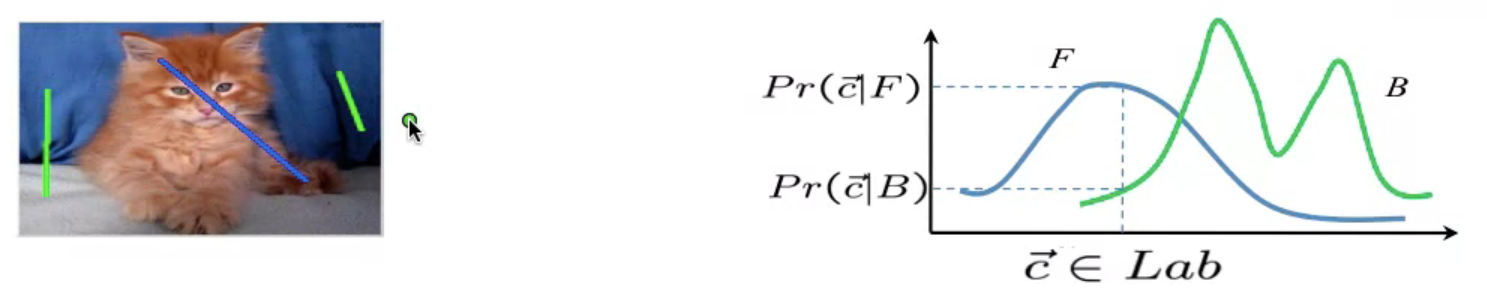
\includegraphics[scale=0.3]{img/cat1.png}
        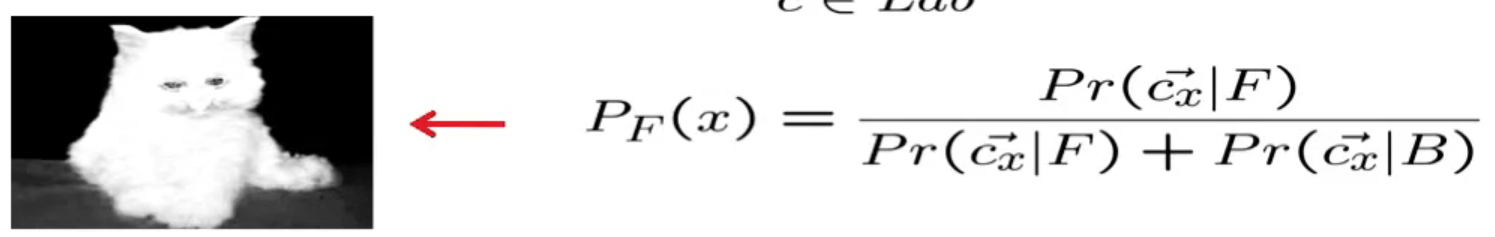
\includegraphics[scale=0.3]{img/cat2.png}
    \end{center}
    The grayscale image of the cat now represents the posterior distribution of which class a pixel is in, where the more white a pixel is, the higher the probability that it is in foreground. But notice that the eyes are very dark, meaning that we classify it as the background. To fix this, we can implement a weighted distance transform, which takes into account the distance between a certain pixel and the foreground/background regions. Let the weighted geodesic distance between two points $s_1, s_2$ be 
    \[d(s_1, s_2) = \min_{C_{s_1 : s_2}} \int_{C_{s_1 : s_2}} W \,ds \]
    which basically looks at all paths $C_{s_1:s_2}$ from $s_1$ to $s_2$, finds the weighted distance across this path, and compute the minimum path. In a discretized space, this is a variant of Dijkstra's algorithm, which can be computed in linear time. The idea is that given a pixel, we want to find the shortest weighted path to a drawn segment, and if the probability of being in the foreground doesn't change too much, it is likely a foreground pixel. This indicates that we want the weight to be 
    \[W = | \nabla P_F (x) \cdot C^\prime_{s_1 : s_2} (x)|\]
    Therefore, we can see the heat map below, where for every point in the image, the distance from that point to the foreground segment (green) is represented to be large if it is red, and small if it is blue. We also do the same for the background segments.
    \begin{center}
        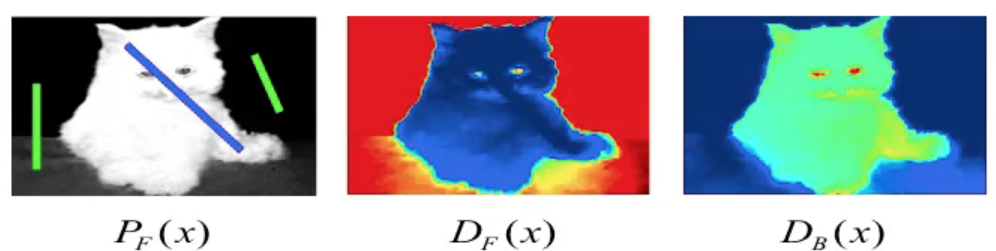
\includegraphics[scale=0.35]{img/cat3.png}
    \end{center}
    Therefore, at a certain point, we compute the shortest weighted paths between the foreground and background segments and choose which ever one is shorter. Once you do this, you take the set of all point where the probabilities of being in the foreground and background are equal, and we are done. 

    The final step is to refine this estimate. With our first order estimate, we can create a narrow band and new scribbles, where the band boundaries serve as the new ``user-inputted" scribbles, and do the same thing over again. Since this new scribble is close to the boundary, it should have more information than our initial guess. This can be done locally as well, with a sliding window that goes around each portion of the boundary. 
    \begin{center}
        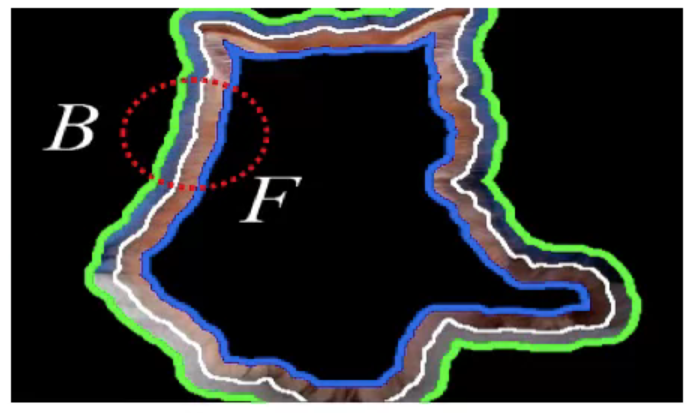
\includegraphics[scale=0.3]{img/cat4.png}
    \end{center}

  \subsection{Graph Cuts}

    Another way to segment images is to construct an underlying graph between the pixels, which acts as nodes, and are connected to their 4-neighbors. We add in a foreground source node and a background sink node, and from the user input. We also want the weights between neighboring nodes to be a function of the gradient between them, encouraging similar pixels to stay in the same group with high weights (and weights between a foreground and background node to be weak). Now we want to partition the graph with a mincut algorithm (which can be solved in polynomial time). 
    \begin{center}
        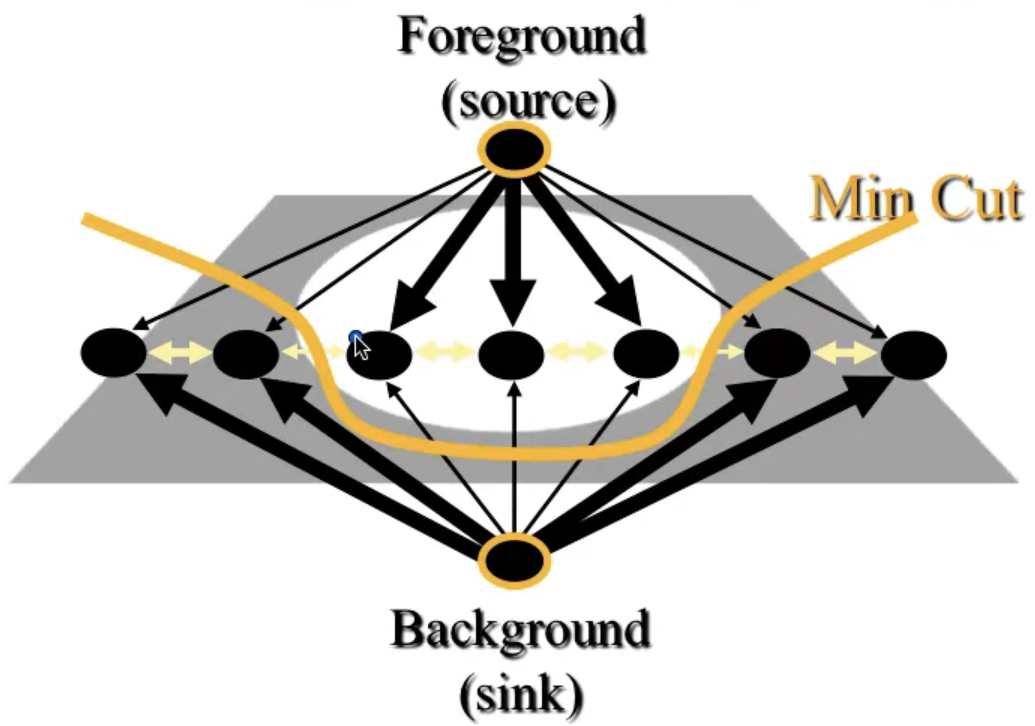
\includegraphics[scale=0.3]{img/mincut.png}
    \end{center}
    This method is actually implemented in MS office. 

  \subsection{Mumford Shah}

    Mumford Shah is really just a regularized optimization algorithm. Given an image $f$, we want to create another image $g$ such that the MSE loss is minimized. However, this just means that $g = f$, but now we add a penalty term that says if we have too many edges, this is penalized. So, doing edge detection on the original image will give us a lot of edge pixels, which will penalize it highly, and so we want a lower dimensional representation $g$ of $f$ such that when we do edge detection on $g$, there won't be many edge pixels. 
    \begin{center}
        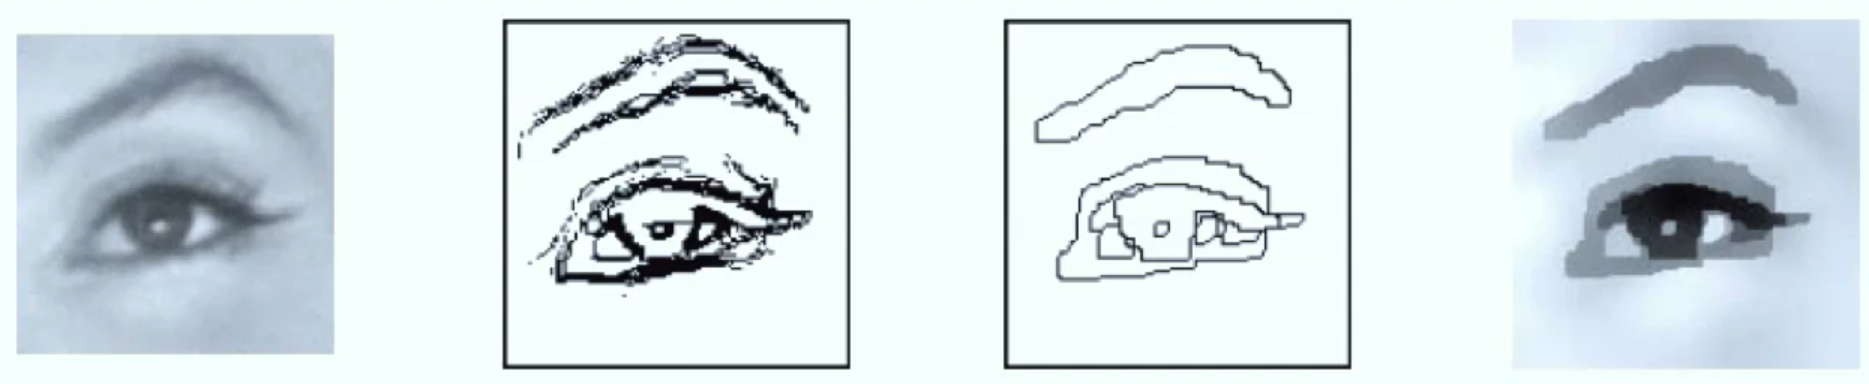
\includegraphics[scale=0.2]{img/mumfordshah.png}
    \end{center}

  \subsection{Active Contours}

    The purpose of active contours is that we want to draw a contour around an object in an image, and it will ``shrink" with a certain velocity until it detects a large change in the gradient of the pixel values, where it will stop. Hyperparameters that determine the momentum can be implemented to get different contours. 
    \begin{center}
        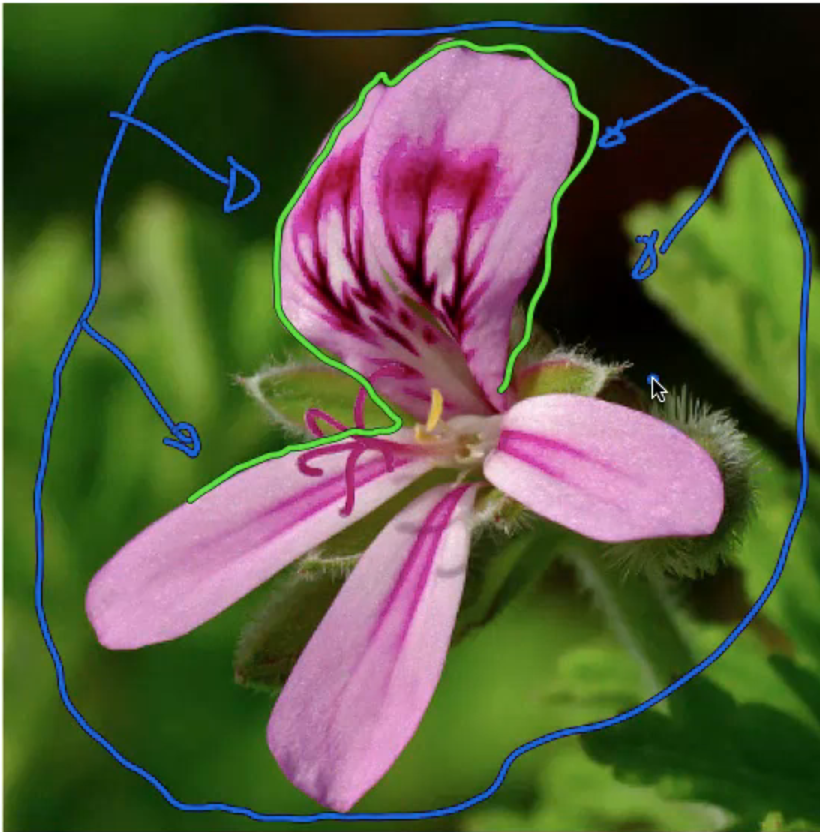
\includegraphics[scale=0.2]{img/active_contours.png}
    \end{center}

\section{PDEs in Image Processing}

    Before, we considered images and videos as inherently discrete objects due to their representation in computers. The PDE point of view says that images are continuous objects, and image processing is the result of iterations of infinitesimal operations. We can also do differential geometry on images and then implement them using numerical analysis. 

    \begin{definition}
    Define $C: [0, 1] \rightarrow \mathbb{R}^2$ as a planar curve, which is closed if $C(0) = C(1)$. Then, we can define the unit tangent vector as 
    \[\mathbf{t}(p) = \frac{C^\prime (p)}{|| C^\prime (p)||} = \frac{C_p|}{||C_p||} = C_s\]
    We know that $||C_s|| = 1$, and so 
    \[\frac{\partial}{\partial s} \langle C_s, C_s \rangle = \frac{\partial}{\partial s} 1 = 0 \implies 2 \langle C_s, C_{ss} \rangle = 0 \implies C_ss \perp C_s\]
    where $C_ss = C^{\prime\prime} (s)$ is the second derivative that describes how the tangent vector is moving, also perpendicular to the curve. We define the \textbf{curvature} as
    \[\kappa = ||C^{\prime\prime} (s) ||\]
    \end{definition}

    Now the \textbf{arclength} $s \mapsto C(s)$ is a parameterization of the curve $C$ that gives us a constant unit tangent vector when differentiating. At every point $\kappa(s)$ is the curvature, and it is intuitive to see that the curvature is preserved under any Euclidean transformation (rotation + translation). There are other \textbf{differential invariants}, defined in Cartan's theorem. To construct this arclength, you must make sure that the speed is constant. 

    But in camera projections, we must take into account affine transformations that comes from tilting. An affine transform that has unit determinant is called \textbf{equi-affine}. To create an arclength that preserves the same differential invarants under affine transformations, you must create a parameterization that preserves the area. 


    \begin{definition}[Surface]
    A surface 
    \[S(u, v) = \{x(u, v), y(u, v), z(u, v)\}\]
    has the normal vector 
    \[\mathbf{N} = \frac{S_u \times S_v}{||S_u \times S_v||}\]
    the area element is $dA = |S_u \times S_v|$, with the total area being 
    \[A = \iint |S_u \times S_v| \, du\,dv \]
    \end{definition}

    Now given a point $p \in \mathbb{R}^3$ on $S$, we can take all paths $C$ that go through $p$. The normal curvature is simply $\langle C_{ss} , \mathbf{N}\rangle$, and the principal curvatures are 
    \begin{align*}
        \kappa_1 & = \max_\theta (\kappa) \\
        \kappa_2 & = \min_\theta (\kappa) 
    \end{align*}
    where $\kappa$ represents all the possible curvatures of all paths at that point. The mean and Gaussian curvatures are defined 
    \begin{align*}
        H & = \frac{\kappa_1 + \kappa_2}{2} \\
        K & = \kappa_1 \kappa_2
    \end{align*}

  \subsection{Curve Evolution}

    Given a curve $C(p)$ parameterized by function $p: [0, 1] \rightarrow [0, 1]$, we can use a partial differential equation to model how it evolves through time. 
    \[\frac{\partial C(p)}{\partial t} = \mathbf{V} (p, t) \iff C_t = \mathbf{V}\]

    An important property is that tangential components do not affect the geometry of an evolving curve. Only the normal component does. Therefore, we can project the original PDE to 
    \[C_t = \langle \mathbf{V}, \mathbf{n} \rangle \mathbf{n}\]
    \begin{enumerate}
        \item The constant flow equation is 
        \[C_t = \mathbf{n}\]
        simply shrinks a curve by enveloping all disk of equal radius centered along the curve, and then it offsets the curves with a constant motion. This can be interesting since it can change the topology of a curve (a curve can split in two, or it can changes smooth points to sharp ones). 

        \item The Euclidean geometric heat equation is 
        \[C_t = C_{ss} = \kappa \mathbf{n}\]
        This curvature flow takes any simple curve, turns it into a convex shape, and then vanishes at a circular point.  

        \item The affine heat equation is 
        \[C_t = \langle C_{vv} , \mathbf{n} \rangle \mathbf{n} = \kappa^{1/3} \mathbf{n}\]
        This curvature flow first becomes convex and then vanishes at an elliptical point. 
    \end{enumerate}
    \begin{center}
        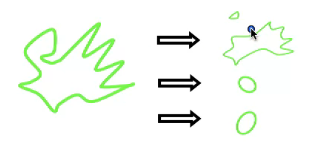
\includegraphics[scale=0.3]{img/3_heat_flows.png}
    \end{center}

    Now to look at \textbf{geodesic active contours}, we can define the PDE 
    \[C_t = \big( g(x, y) \kappa - \langle \nabla g(x, y), \mathbf{n}\rangle \big) \mathbf{n}\]
    where the velocity $\mathbf{v}$ going in the normal direction is the coefficient of $\mathbf{n}$. 

    \begin{definition}[Level Sets]
    We can also represent a closed planar curve as the level set 
    \[C = \{(x, y) \mid \phi(x, y) = 0\}\]
    for some function $\phi$, where the interior of the curve is when $\phi > 0$. Recall that the gradient is normal to the tangent vector of this level set (and we can normalize it by convention). The \textbf{level set curvature} is defined 
    \[\kappa = \mathrm{Div} \bigg( \frac{\nabla \phi}{||\nabla \phi||}\]
    \end{definition}

    The reasons we like to use the level set formulation is that 
    \begin{enumerate}
        \item it handles changes in topology well (since we can just define a function with multiple peaks 
        \item numeric grid points never collide or drift apart 
        \item it is a natural philosophy for dealing with gray level images 
    \end{enumerate}

    Therefore, to implement a curve evolution of form 
    \[\frac{\partial C}{\partial dt} = V \mathbf{N}(t)\]
    we can equivalently define for level sets a function $\phi$ that satisfies 
    \[\frac{\partial \phi}{\partial t} = V |\nabla \phi|\]

  \subsection{Calculus of Variations}

    \begin{definition}
    Calculus of variations is a generalization of calculus that seeks to find a function for which a given functional has a minimum or maxium, i.e. find extrema values of intergals of the form 
    \[\int F(u, u_x) \,dx\]
    It has an extremum only if the Euler Lagrange differential equation is satisfied 
    \[ \bigg( \frac{\partial}{\partial u} - \frac{d}{dx} \frac{\partial}{\partial u_x} \bigg) f(u, u_x) = 0\]
    \end{definition}

    \begin{example}
    Find the shape of the curve $u(x)$ with the shortest length given $u(x_0), u(x_1)$, i.e. that minimizes 
    \[\int_{x_0}^{x_1} \sqrt{1 + u_x^2} \,dx\]
    A differential equation that $u(x)$ must satisfy is 
    \[ \bigg( \frac{\partial}{\partial u} - \frac{d}{dx} \frac{\partial}{\partial u_x} \bigg) f(u, u_x) = 0\]
    and evaluating it gives 
    \[\frac{u_{xx}}{(1 + u_x^2)^{3/2}} \implies u_x = a \implies u(x) = ax + b\]
    i.e. it must be a linear function. 
    \end{example}

  \subsection{Anistropic Diffusion}

    Remember that in Gaussian blurring, we have a symmetric kernel where we can do some blurring by mixing in pixels across edges. Now, anisotropic smoothing tries to average pixel values \textit{within} the boundaries. Therefore, we can remove noise within objects and not have it corrupt the edges. 

    We want to find 
    \[\min_I \int_\Omega \rho(| \nabla I|) \,d \Omega \implies \frac{\partial I(x, y, t)}{\partial t} = \mathrm{div} \bigg( \rho^\prime \frac{\nabla I}{|\nabla I|}\]
    For example, if 
    \begin{enumerate}
        \item $\rho(a) = a$, then 
        \[\min_I \int |\nabla I| \implies I_t = \mathrm{div} \bigg( \frac{\nabla I}{|\nabla I|} \bigg)\]
        which is an isotropic diffusion which moves it in a way according to the curvature of the level lines. 

        \item $\rho(a) = a^2$, then $\rho^\prime(a) = 2a$
        \[\min_I \int |\nabla I|^2 \implies I_t = \mathrm{div} \bigg( 2 |\nabla I| \frac{\nabla I}{|\nabla I|} \bigg) = \text{Laplacian}(I)\]
        and so this is the equation for heat flow, which smooths it in an isotropic fashion. 
    \end{enumerate}

\section{Image and Video Inpainting}

    \textbf{Image inpainting} is a specific problem that refers to modifying an image in a non-detectable form. It can refer to filling in damaged parts, color correcting, or removing objects. Inpainting is everywhere, in biological animals that camoflague or done by ourselves when we fill in the blind spots in our visual systems. 

  \subsection{Inpainting via PDEs}

    It turns out that professional conservators inpaint by continuing boundaries within the region of interest, then filling in colors, and finally adding noise. 
    \begin{center}
        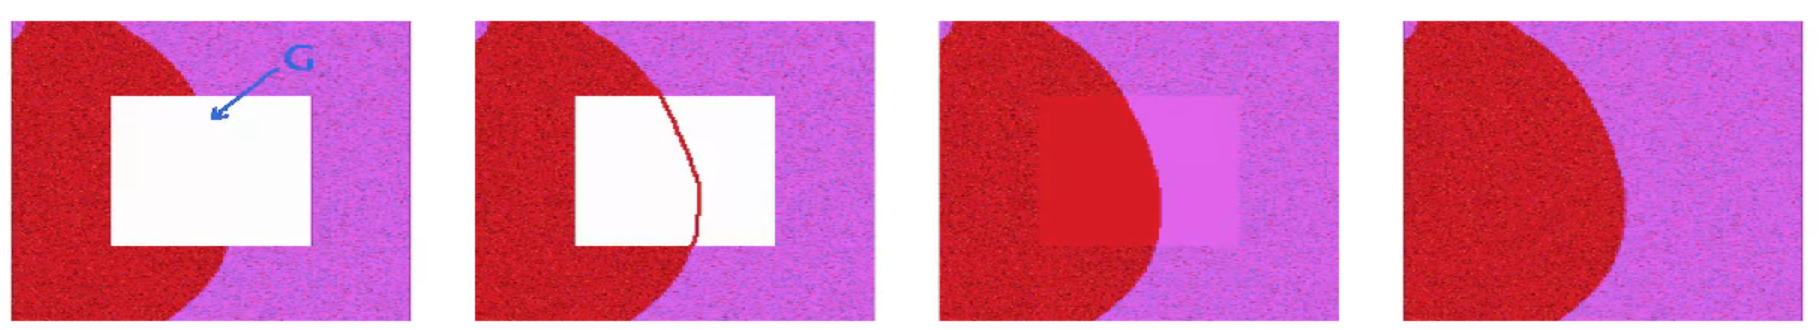
\includegraphics[scale=0.2]{img/inpainting.png}
    \end{center}
    This sort of looks like some water that is filling up the regions, which we can emulate with a PDE.

\end{document}
